%%%%%%%%%%%%%%%%%%%%%%%%%%%%%%%%%%%%%%%%%%%%%%%%%%%%%%%%%%%%%%%%%%%%%%%%%%%%
% AGUJournalTemplate.tex: this template file is for articles formatted with LaTeX
%
% This file includes commands and instructions
% given in the order necessary to produce a final output that will
% satisfy AGU requirements, including customized APA reference formatting.
%
% You may copy this file and give it your
% article name, and enter your text.
%
%
% Step 1: Set the \documentclass
%
%



%% EGU 2-column papers and preprints
\documentclass[nhess, manuscript]{copernicus}
%% AGU
%\documentclass[draft]{agujournal2019}
%\draftfalse
%\journalname{Geophysical Research Letters}

%\usepackage[german, english]{babel}
\usepackage{tabularx}
%\usepackage{cancel}
%\usepackage{multirow}
%\usepackage{supertabular}
%\usepackage{algorithmic}
%\usepackage{algorithm}
%\usepackage{amsthm}
\usepackage{float}
%\usepackage{rotating}
\usepackage[percent]{overpic}
\usepackage{contour}

\contourlength{.1em}% default is 0.03em

%\usepackage{url} %this package should fix any errors with URLs in refs.
%\usepackage{lineno}
%\usepackage[inline]{trackchanges} %for better track changes. finalnew option will compile document with changes incorporated.
%\usepackage{soul}
%\linenumbers

%CMZ
%\usepackage{natbib}
%\usepackage{xcolor}
%\usepackage{graphicx}
%\newcommand{\degree}{$^{\circ}$}
%\newcommand{\texttilde}{$\sim$}
%\usepackage{tabularx}
%\renewcommand\tabularxcolumn[1]{m{#1}}% for vertical centering text in X column

%%%%%%%
% As of 2018 we recommend use of the TrackChanges package to mark revisions.
% The trackchanges package adds five new LaTeX commands:
%
%  \note[editor]{The note}
%  \annote[editor]{Text to annotate}{The note}
%  \add[editor]{Text to add}
%  \remove[editor]{Text to remove}
%  \change[editor]{Text to remove}{Text to add}
%
% complete documentation is here: http://trackchanges.sourceforge.net/
%%%%%%%







\begin{document}

\Author[1]{Colin M.}{Zarzycki}
\Author[1,*]{Benjamin D.}{Ascher}
\Author[2]{Alan M.}{Rhoades}
\Author[3]{Rachel R.}{McCrary}

\affil[1]{Department of Meteorology and Atmospheric Science, The Pennsylvania State University, University Park, PA, USA}
\affil[2]{Climate and Ecosystem Sciences Division, Lawrence Berkeley National Laboratory, Berkeley, CA, USA}
\affil[3]{NSF, National Center for Atmospheric Research, Research Applications Laboratory, Boulder, CO, USA}
\affil[*]{now at Colorado State University}

\correspondence{Colin M. Zarzycki (czarzycki@psu.edu)}

\title{Algorithmically Detected Rain-on-Snow Flood Events in Different Climate Datasets: A Case Study of the Susquehanna River Basin}
% Alternative titles
%Using the Susquehanna River Basin as an example in how algorithmically detected rain-on-snow flood events differ in climate data
%Algorithmically Detected Rain-on-Snow Flood Events in Different Climate Datasets: A Case Study of the Susquehanna River Basin
%Exploring the Variability of Algorithmically Detected Rain-on-Snow Flood Events in Different Climate Datasets: A Case Study of the Susquehanna River Basin

\runningtitle{Algorithmic detection of basin-scale rain-on-snow events}

\runningauthor{Zarzycki}

\received{}
\pubdiscuss{} %% only important for two-stage journals
\revised{}
\accepted{}
\published{}

\firstpage{1}

\maketitle

\begin{abstract}
Rain-on-snow (RoS) events in regions of ephemeral snowpack -- such as the northeastern United States -- can be key drivers of cool-season flooding. We describe an automated algorithm for detecting basin-scale RoS events in gridded climate data by generating an area-averaged time-series and then searching for periods of concurrent precipitation, surface runoff, and snowmelt exceeding pre-defined thresholds. When evaluated using historical data over the Susquehanna River Basin (SRB), the technique credibly finds RoS events in published literature and flags events that are followed by anomalously high streamflow as measured by gage data along the river. When comparing four different datasets representing the same 21-year period, we find large differences in RoS event magnitude and frequency, primarily driven by differences in estimated surface runoff and snowmelt. Using dataset-specific thresholds improves agreement between datasets but does not account for all discrepancies. We show that factors such as meteorological forcing and coupling frequency as well as choice of land surface model play roles in how data products capture these compound extremes and suggest care is to be taken when climate datasets are used by stakeholders for operational decision-making.
\end{abstract}

% \section*{Plain Language Summary}
% Rain-on-snow events happen when rain falls on existing snowpack, leading to rapid snowmelt and potential flooding during the cool season of the northeastern United States. We developed a new method to identify these events using climate data without the need for classification by hand, allowing us to calculate statistics regarding rain-on-snow occurrence. By analyzing historical data over the Susquehanna River Basin, this technique successfully identified known rain-on-snow events that led to increases in river flow and associated flooding. We compared four different historical datasets. Even though all datasets represent the same period, we found variations in the frequency and severity of how rain-on-snow events are captured due to differences in how developers apply weather conditions to determine snowmelt and runoff. Our findings underscore the importance of selecting appropriate climate data for studying such events. This is crucial for effective flood management and decision-making, ultimately aiding in the development of better tools for anticipating and handling the risks associated with compound extremes.

%% Sub 500 characters
%We developed an automated workflow to detect rain-on-snow events, which cause flooding in the northeastern U.S., in climate data. Analyzing the Susquehanna River Basin, this technique identified known events affecting river flow. Comparing four gridded datasets revealed variations in event frequency and severity, driven by different snowmelt and runoff estimates. This highlights the need for accurate climate data in flood management and risk prediction for these compound extremes.

\introduction

Rain-on-snow (RoS) events have been increasingly studied over the past few decades, yet such research is overwhelmingly focused on mountainous regions with well-defined seasonal snowpacks \citep{singh1997hydrological,mccabe2007rain,wayand2015modeling,sterle2019hydroclimate,musselman2018projected,poschlod2020climate,Hatchett2021,siirila2021a,heggli2022toward,yu2022diverse,brandt2022a,maina2023diverging,haleakala2023watershed}.
Correspondingly, there has been less focus in areas with more ephemeral snow cover, such as the northeastern United States (US), even though RoS events, a flavor of compound extreme \citep{aghakouchak2020climate}, produce many cases of `slow-rise' flooding -- floods generally occurring more than six hours after the onset of the meteorological driver \citep{dougherty2021high}.
Climatologically, RoS events in the northeastern US peak in late winter and spring \citep{ashley2008flood,villarini2010flood,dougherty2019climatology,wachowicz2020rain} and are key drivers of flooding in New England and the Atlantic side of Canada \citep{collins2014annual}.
Synoptic case study analyses of recent RoS events in the mid-Atlantic highlight inland-running extratropical cyclones that advect warm, moist air into the region as key dynamical drivers \citep{grote2021synoptic,suriano2023atmospheric}.
Rapid snow ablation in ephemeral snow regions has been shown to have a strong correlation with increases in basin streamflow in the days following snowmelt \citep{suriano2020discharge,suriano2023atmospheric}.

While climatological studies are critically important, event-level analysis has become increasingly valuable when communicating climate risks \citep{shepherd2018storylines}.
One river basin in the northeastern US that has historically dealt with RoS events is the Susquehanna River Basin (SRB) -- a basin home to more than four million people \citep{leathers2008hydroclimatic} and one considered climatologically flood-prone due to the wide variety of weather phenomena that occur within the region \citep{perry2000significant}.
The most consequential non-tropical-cyclone flood in recent SRB history was a RoS flood that occurred in January 1996, resulting in $\sim$\$1.5 billion in damages and 30 fatalities \citep{leathers1998severe}. Significant events such as this are frequently used by stakeholders as a point of reference for real-time forecasts and long-term planning \citep{george2019the}.
Other evidence, such as the Great Flood of 1936 (another RoS event) and the fact that sediment records indicate prehistoric periods of high flood activity are associated with negative phases of the North Atlantic Oscillation (NAO) (which drive positive snowpack anomalies in the northeastern US, \citep{hartley1998synoptic}) underscore the importance of these events to regional hydrology \citep{toomey2019the}.

While studying historical events is important for planning purposes, and historical reforecasts using imposed warming approaches can provide clues as to how similar events may unfold in the future (e.g., \citet{pettett2023the}), it is difficult for such approaches to provide risk quantification from a frequency-of-occurrence perspective. For these climatological evaluations, it is desirable to be able to identify such events in both observational datasets and model simulations, including future climate projections.
Unfortunately, assessing extreme, compound, and discrete events in climate data sets is a complex challenge, particularly because such datasets are not necessarily developed specifically for this purpose \citep{angelil2017an,parker2020model} and there is commonly a lack of observational reference datasets to quantify their fidelity.
Gridded datasets (spatiotemporally continuous data provided on a regular latitude-longitude mesh) of the historical record are frequently used to assess hydrometeorological extremes in locations with poor or non-existent station observations and climate analyses requiring multiple complex variables in addition to evaluating model sensitivity and performance.
Further, future changes in RoS event frequency and character due to climate change are projected via the use of free-running models, which operate on numerical grids and don't have an \textit{a priori} record to compare to, making the use of an automated heuristic a requirement.

Therefore, to extract information regarding compound hydrometeorological extremes, such as RoS events, and their corresponding statistics, algorithmic techniques that objectively analyze datasets without manual intervention are desirable.
Here, we demonstrate a technique for generating a RoS event database at the basin scale for arbitrary gridded datasets and intercompare key decision-relevant differences (e.g., flood frequency) across four climate data products.
We choose to focus on the SRB based on its proximity to major population centers, existing evidence for increasing flood hazards and exposure in the basin \citep{sharma2021regional}, and the aforementioned 1996 extreme event serving as a benchmark for the mid-Atlantic US, although the technique described can be applied to any geographically defined basin with properly specified thresholds.

%We focus on the direct prediction of coupled surface processes (i.e., snow water equivalent and surface runoff) to minimize issues with statistical or dynamical downscaling and permit a like-to-like comparison between different datasets.

\section{Methods}

\subsection{Datasets}

We evaluate RoS events within three widely-used climate datasets and in one state-of-the-art Earth system model (ESM) nudged towards an atmospheric reanalysis.
All four datasets seek to reproduce observed conditions, although each uses a distinct methodology to do so.
First, we investigate the dataset described in \citet{livneh2015spatially} (hereafter, L15).
L15 is a widely-used 1/16\degree{} hydrometeorological dataset covering most of North America.
Meteorological data provided by L15 consists of daily precipitation, temperature (maximum and minimum), and wind speed at each location \citep{henn2018an}.
This data is then temporally interpolated to obtain subdaily estimates \citep{bohn2013global}, which are then used to drive the Variable Infiltration Capacity (VIC, \citet{liang1994simple}) land surface model (LSM) to produce hydrometeorological outputs.
Next, we investigate the 1/8\degree{} North American Land Data Assimilation System (NLDAS-VIC4.0.5)  described in \citet{xia2012continental1}.
NLDAS is driven by offline atmospheric forcing derived from the North American Regional Reanalysis, with adjustments made to some variables based on observations.
NLDAS uses a combination of daily observations and radar data to produce hourly estimates of precipitation.
While there are multiple NLDAS-2 LSMs that produce hydrologic output variables, we analyze only the NLDAS-VIC4.0.5 as it is the most methodologically consistent with L15.
We also analyze a $\sim$0.5\degree{} global reanalysis (JRA-55, \citet{kobayashi2015jra55}), generated by running a prognostic ESM while continually assimilating observational data during integration.
Global reanalyses serve as a bridge between in-situ, but spatio-temporally unstructured, observational data and free-running climate models \citep{parker2016reanalyses}.
Finally, a $\sim$1\degree{} nudged version of the U.S. Department of Energy (DOE) Energy Exascale Earth System Model (E3SM, \citet{golaz2022the}) model is analyzed \citep{zhang2022further}. Assessing this dataset provides insight into the capability of ESMs used in climate assessments (e.g., the Coupled Model Intercomparison Project Phase 6 (CMIP6), \citet{eyring2016overview}) to capture observed hydrometeorological extreme events.
E3SM performs close to the CMIP6 ensemble mean across several measures of skill \citep{Fasullo2020}.
To constrain the large-scale meteorology in E3SM to match observed conditions, the E3SM simulation is nudged using 6-hourly fields from the ERA5 reanalysis \citep{hersbach2020era5} generated using the technique contained in the Betacast toolkit, initially outlined in \citet{zarzycki2015experimental}.
This nudging acts as a crude assimilation technique and is only applied in the free atmosphere (above nominally 850 hPa, or 1 kilometer). The zonal and meridional winds are nudged to ERA5 analysis with a relaxation timescale $\tau$ = 3 hours and the temperature is nudged with $\tau$ = 24 hours. No nudging is performed on the surface pressure or moisture fields.
The simulation reproduces observed patterns of 500 hPa geopotential height and sea level pressure while simulating grid-scale processes relatively untethered by the nudging reanalysis product \citep{sun2019impact}.
E3SM is run with a spectral element dynamical core on an unstructured cubed-sphere mesh ($n_e$30$n_p$4) and simulation output is remapped to a 1\degree{}x1\degree{} rectilinear grid using higher-order methods \citep{hill2004architecture}. All model settings and tunings are left as the default contained in the commit used here (f9cbe57).

\subsection{Defining basin-scale events}

To identify RoS events, three hydrometeorological variables are extracted over the SRB.
These include precipitation (PRECIP), snow water equivalent (SWE), and surface water runoff (ROF).
The 24-hour change in SWE from the previous day (dSWE) is calculated via a simple backward difference.
All data is standardized to daily average values (00Z to 00Z) by temporally averaging any sub-daily (e.g., hourly) data at each grid cell.
Grid cells that have at least 50\% of their area enclosed by the boundary of the SRB are kept, while those exterior to the SRB are set to missing values.
The resulting domains for each product can be seen in Fig. \ref{fig:means}. A basin-wide time series is then constructed by spatially averaging fields for each day and smoothing the resulting time series using a moving average to reduce day-to-day noise.
We choose a 5-day window based on mid-latitude synoptic timescales \citep{holton2004introduction}, although other window durations did not materially impact these findings (not shown).

This results in a one-dimensional time series with a single value for each calendar day that represents the SRB basin-averaged conditions for each data product.
RoS days are defined by flagging periods of negative dSWE and positive ROF that both exceed specified thresholds ($t$) on the same days.
Contiguous days are considered to be part of a single `event' such that discrete events can last for different durations.
We test two methods of thresholding; one uses fixed thresholds across all four datasets (FIXED) and the other defines dataset-specific thresholds by those exceeding 95\% of all daily values (RELATIVE).
For FIXED, we require an average dSWE of -1.4 mm/day ($t_{\textrm{dSWE}}$) and ROF of 1.4 mm/day ($t_{\textrm{ROF}}$) averaged across the SRB based on a manual sensitivity analysis.
Thresholds in the RELATIVE configuration are calculated independently for each dataset by setting the threshold to the 95\% value of its own 1985-2005 time series.
To enforce a criterion that precipitation occurs during at least some portion of the event, we require an average PRECIP of 2 mm/day ($t_{\textrm{PRECIP}}$), which is kept the same in both the FIXED and RELATIVE configurations. We note that our findings are actually largely insensitive to the magnitude of the PRECIP threshold (or even its inclusion), implying the vast majority of events with high dSWE and ROF are also associated with non-zero PRECIP.
This supports the notion that similar synoptic meteorological patterns \citep{grote2021synoptic} and additional liquid input to the surface (i.e., runoff being a combination of snowmelt and water flux from the atmosphere) lead to the majority of RoS floods being associated with, at least, some precipitation versus precipitation alone being a primary driver of such events.
It also concurs with \citet{suriano2023atmospheric}, who found that, while RoS days contributed disproportionately to extreme snow ablation events, snowmelt also occurred in a myriad of non-precipitating patterns, including high-pressure overhead and under northwesterly/westerly large-scale flow.
We argue this also corroborates the finding that actual heat transfer between the liquid rain and the surface of the snowpack is rather small and explains only a small fraction of the observed snowmelt \citep{moore1984controls}.

For context, our definition here of RoS is somewhat arbitrary. Most studies enforce some fixed combination of precipitation and snowpack threshold. \citet{ye2008winter} classified events as liquid precipitation falling onto at least 10 mm of existing snowpack in a gridbox. \citet{musselman2018projected} define `RoS days' where at least 10 mm of precipitation falls on at least 10 mm of snowpack in a given day. This technique was adopted by \citet{lopez2021changes} and \citet{maina2023diverging}. A similar strategy, but applying higher thresholds (20 mm precipitation, 250 mm snowpack), was used by \citet{wurzer2016influence}. Likewise, \citet{hotovy2023changes} required 10 mm of existing SWE and greater than 0\degree{}C surface temperatures to enforce collocated daily precipitation (of at least 5 mm) to fall in liquid form. Instead of a SWE metric, others have applied snow cover fraction or some other snow/no-snow classification in addition to a precipitation threshold \citep{mazurkiewicz2008assessing,pradhanang2013rain,cohen2015trends}. Others include some measure of snowmelt, such as \citet{freudiger2014large} and \citet{li2019the} who required 3 mm of rainfall, 10 mm SWE, and a 20\% reduction in the snowpack (implied dSWE $<=$ -20 mm/day). \citet{suriano2022north} similarly required a 10 mm daily snow depth decrease that occurred in combination with above-freezing temperatures and non-zero precipitation. However, relative strategies have also been proposed, such as the 98\% threshold used for covarying extremes in the compound event analysis of \citet{poschlod2020climate}. Other studies simply require the joint occurrence of precipitation and snowmelt in a given period \citep{mccabe2007rain,surfleet2013variability,collins2014annual,guan2016hydrometeorological,jeong2018rain}. \citet{wachowicz2020rain} used the same gridded data and explored four different definitions derived from some of the above and found high-level agreement.

This brief literature review is not meant to be considered exhaustive, but rather to highlight that both RoS evaluation techniques in this manuscript fall within the scope of existing strategies. It also emphasizes that extreme RoS events in mountainous regions with more seasonal snowpack or those using gridpoint values versus basin-integrated metrics may require different thresholds. With the caveat that much of the previously cited RoS work has focused on regions with less ephemeral snowpack (e.g., western U.S. mountains), the algorithm discussed here falls within the envelope of previously published results both from a heuristic perspective and also with respect to our defined thresholds.

Lastly, to show all datasets adequately represent the same period, Pearson correlations of basin-wide statistics (Table \ref{table:correlations}) were statistically significant with a two-sided $t$-test between all permutations of daily time series. This confirms that all datasets fundamentally represent the same meteorology and land surface evolution as processed here and can therefore be directly compared to one another.

\begin{table}[]
\caption{Pearson correlations between data products for daily timeseries of precipitation (top), surface runoff (middle), and 24-hour change in snow water equivalent (bottom) over the study period. All values are correlated significantly at greater than the 99.9\% confidence level using a two-sided $t$-test, indicating that all timeseries represent the same historical period and include relevant day-to-day variations over the SRB.}
\begin{tabular}{lcccc}
 \hline
      &      & PRECIP &       &       \\ \hline
      & JRA  & L15    & NLDAS & E3SM \\
JRA   & 1.00 & 0.76   & 0.89  & 0.75 \\
L15   & 0.76 & 1.00   & 0.81  & 0.93 \\
NLDAS & 0.89 & 0.81   & 1.00  & 0.77 \\
E3SM  & 0.75 & 0.93   & 0.77  & 1.00  \\ \hline \hline
      &      & ROF    &       &      \\ \hline
      & JRA  & L15    & NLDAS & E3SM \\
JRA   & 1.00 & 0.89   & 0.88  & 0.83 \\
L15   & 0.89 & 1.00   & 0.85  & 0.74 \\
NLDAS & 0.88 & 0.85   & 1.00  & 0.82 \\
E3SM  & 0.83 & 0.74   & 0.82  & 1.00 \\ \hline \hline
      &      & dSWE   &       &      \\ \hline
      & JRA  & L15    & NLDAS & E3SM \\
JRA   & 1.00 & 0.34   & 0.46  & 0.47 \\
L15   & 0.34 & 1.00   & 0.79  & 0.66 \\
NLDAS & 0.46 & 0.79   & 1.00  & 0.71 \\
E3SM  & 0.47 & 0.66   & 0.71  & 1.00 \\ \hline \hline
\end{tabular}
\label{table:correlations}
\end{table}

\section{Results}

\subsection{Climatology}

We first investigate the mean climatology of relevant quantities over the SRB to provide some context into each data product's baseline.
The average cool-season (November-April, inclusive) distributions of PRECIP, ROF, SWE, and dSWE are shown in Fig. \ref{fig:means}.
The higher resolution of L15 and NLDAS is evident from the added structure in the mean fields of the first two columns.
Mean PRECIP (Fig. \ref{fig:means}a-d) is higher in JRA and E3SM when compared to the L15 and NLDAS.
This may be due to factors such as atmospheric model biases or the inclusion of rain gauge data in L15 and NLDAS, although it has been shown that significant spread exists in historical gridded climate data products, even for more commonly observed variables such as precipitation \citep{gutmann2012comparison,livneh2014filling,henn2018an}.
ROF (Fig. \ref{fig:means}e-h) and SWE (Fig. \ref{fig:means}i-l) climatologies differ between the data products.
Notably, L15 produces mean ROF values that are less than half of the climatologies of each of the other three datasets.
It is well-known that simulated ROF from different hydrologic models can be extremely variable, with regional differences between products reaching an order of magnitude \citep{gudmundsson2012comparing,sood2015global,beck2017global}.
NLDAS produces less SWE climatologically, $<$20\% of the SWE produced by L15 or E3SM, and even less than the coarser JRA product.
Previous work has also shown that SWE estimates can vary greatly across datasets \citep{lundquist2015high,Rhoades2018a}, particularly over the ephemeral snow area of the northeastern U.S. \citep{mccrary2017evaluation,mccrary2022projections}.
dSWE climatology is shown in Fig. \ref{fig:means}m-p.
When calculating the mean, all accumulation (or zero change) days are ignored to isolate only days where snow loss occurred.
Here, NLDAS also exhibits the lowest magnitude of dSWE, although we speculate this is at least partly due to the shallower mean snowpack.
The largest climatological dSWE magnitude is found in JRA, even though the SWE does not contain the largest depths, implying the snowpack is more variable in JRA and may be prone to more rapid snow loss (from a dSWE per unit time perspective).

We emphasize that, from a physical standpoint, differences in snowfall and snowmelt timing \citep{rauscher2008future,mccabe2005trends}, snow properties \citep{brown2006evaluation}, temperature and permeability of the soil \citep{niu2006effects}, precipitation type partitioning \citep{knowles2006trends}, and evapotranspiration \citep{zheng2019on} all can lead to differences in how these quantities are simulated.
We speculate that these mechanisms are playing important roles in the differing mean climatologies but performing a fully-detailed water budget analysis for each of the land surface models leveraged by these datasets is beyond the scope of this analysis.

\subsection{Flagged event statistics}

Turning to the algorithmically flagged RoS events, Table \ref{table:means} shows summary statistics for all four data products.
Focusing on the FIXED thresholds, the total number of discrete events that occurred in the SRB over the 21-year study period varies by an order of magnitude, from 6 events in L15 to 58 in E3SM.
Interestingly, large differences don't necessarily appear when considering the mean event-averaged dSWE, ROF, or PRECIP (last three columns).
In fact, when a RoS event occurs, L15 has the largest PRECIP$_{\textrm{a}}$ and largest dSWE$_{\textrm{a}}$, although the smallest ROF$_{\textrm{a}}$.

When using the RELATIVE thresholds, the event frequencies agree better, with only a factor of two difference between L15/NLDAS and JRA/E3SM.
The number of events in L15 increases because the ROF threshold (95th percentile of daily values) is reduced from 1.4 to 0.6 mm/day.
Similarly, the dSWE threshold magnitude is reduced from -1.4 mm/day to -0.8 mm/day in NLDAS.
Conversely, fewer events were classified in E3SM, due to increases in both the required ROF and dSWE thresholds applied to the daily climatology.
However, even when accounting for the baseline climatological differences of the data products by thresholding on percentiles, rather than absolute magnitudes, differences still are evident in all metrics.

\begin{figure}
\begin{tabular}{c}
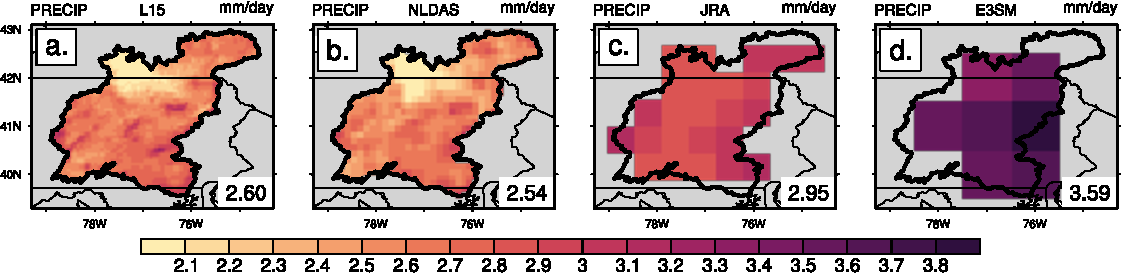
\includegraphics[width=0.98\linewidth]{{figs/cropped/climo_comp_panel_PRECIP}.pdf} \\
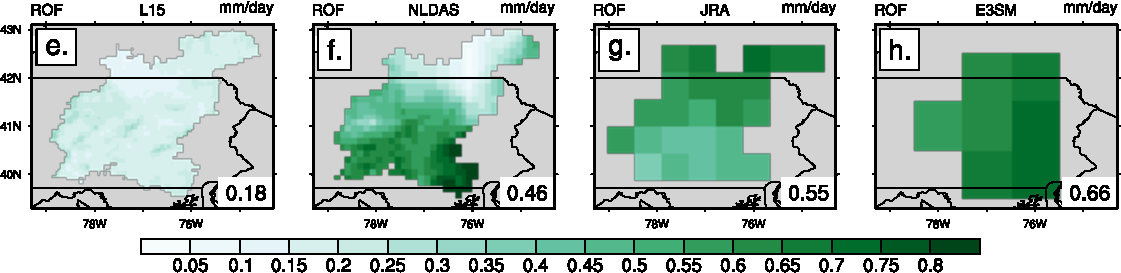
\includegraphics[width=0.98\linewidth]{{figs/cropped/climo_comp_panel_ROF}.pdf} \\
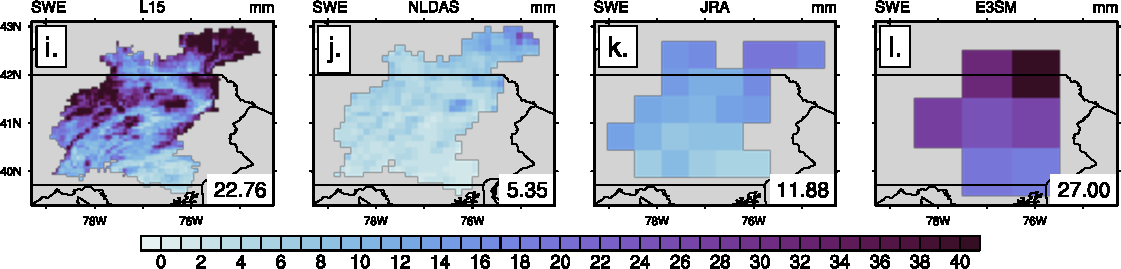
\includegraphics[width=0.98\linewidth]{{figs/cropped/climo_comp_panel_SWE}.pdf} \\
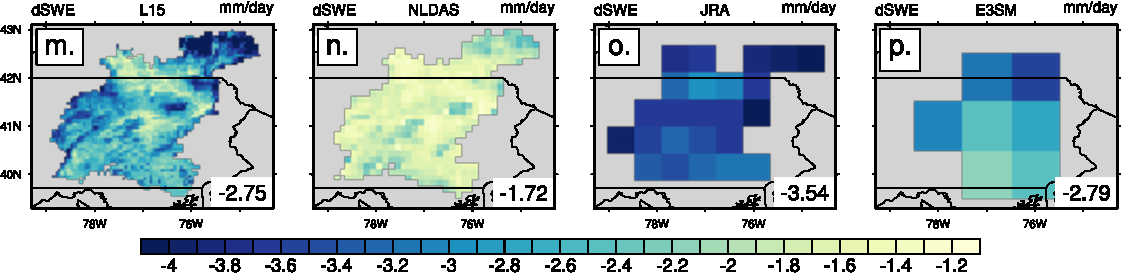
\includegraphics[width=0.98\linewidth]{{figs/cropped/climo_comp_panel_dSWE}.pdf}
\end{tabular}
\caption{November to April (inclusive) mean climatologies of L15, NLDAS, JRA, and E3SM (left to right). From top to bottom are precipitation (PRECIP; mm/day), surface runoff (ROF; mm/day), snow water equivalent (SWE; mm), and daily change in snow water equivalent (dSWE; mm/day). dSWE only includes days with snow loss at a particular grid cell. Data is only included if $>$50\% of a grid cell lies within the SRB bounds (black outline).}
\label{fig:means}
\end{figure}

\begin{table}
\caption{Statistics of RoS events over the SRB using FIXED thresholds (top) and RELATIVE thresholds (bottom). $t_{\textrm{dSWE}}$, $t_{\textrm{ROF}}$, and $t_{\textrm{PRECIP}}$ represent the thresholds used for snow water equivalent loss, surface runoff, and precipitation, respectively (mm/day). Events represent the number of RoS events flagged over the 1980-2005 period. Duration is the average number of consecutive days an RoS event lasts. dSWE$_{a}$, ROF$_{a}$, and PRECIP$_{a}$ represent the average snow loss, amount of runoff rate, and amount of precipitation rate (mm/day) per event by calculating the mean daily value for each individual event and then averaging those.}
\begin{tabular}{lcccccccc}
      &  $t_{\textrm{dSWE}}$ & $t_{\textrm{ROF}}$ & $t_{\textrm{PRECIP}}$ & Events & Duration & dSWE$_{a}$ & ROF$_{a}$ & PRECIP$_{a}$ \\
      &  \textit{mm day$^{-1}$} & \textit{mm day$^{-1}$} & \textit{mm day$^{-1}$} & \textit{\#} & \textit{days} & \textit{mm day$^{-1}$} & \textit{mm day$^{-1}$} & \textit{mm day$^{-1}$} \\ \hline
FIXED &         &         &         &     &              &              &                &                \\ \hline
L15   & -1.4     & 1.4     & 2.0     & 6   & 3.2          & -5.3          & 1.5            & 9.5            \\
NLDAS & -1.4     & 1.4     & 2.0     & 16  & 2.9          & -5.2          & 2.1            & 6.3            \\
JRA   & -1.4     & 1.4     & 2.0     & 48  & 3.5          & -4.4          & 2.6            & 5.3            \\
E3SM  & -1.4     & 1.4     & 2.0     & 58  & 4.1          & -5.2          & 2.4            & 6.5            \\ \hline
RELATIVE      &         &         &         &     &              &              &                &                \\ \hline
L15   & -1.5     & 0.6     & 2.0     & 20  & 5.2          & -5.3          & 1.1            & 6.2            \\
NLDAS & -0.8     & 1.4     & 2.0     & 20  & 2.8          & -4.2          & 2.1            & 7.2            \\
JRA   & -1.9     & 1.6     & 2.0     & 40  & 3.2          & -4.1          & 2.5            & 5.1            \\
E3SM  & -2.2     & 1.8     & 2.0     & 41  & 4.1          & -8.0          & 2.9            & 6.9 \\ \hline \hline
\end{tabular}
\label{table:means}
\end{table}

The differences across gridded climate data products are also shown in Fig. \ref{fig:histograms2} (FIXED) and in Fig. \ref{fig:histograms} (RELATIVE). The sign of dSWE is flipped here for ease of visualization with the other metrics (i.e., positive dSWE in both figures denotes snowpack). We focus our discussion on the relative threshold results in Fig. \ref{fig:histograms} for brevity, although note that the distributions of event statistics (Fig. \ref{fig:histograms2}b-d and Fig. \ref{fig:histograms}b-d) are qualitatively similar between the two.

Figure \ref{fig:histograms}a shows the total number of RoS events flagged over the climatological period (fourth column of Table \ref{table:means}), while Fig. \ref{fig:histograms}b-d shows the frequency distribution for basin-averaged maximum rates of PRECIP, ROF, and dSWE at the event level. These are calculated by selecting the maximum daily value from the array of actual (i.e., unsmoothed) daily values during each RoS event.

The maximum PRECIP associated with flagged RoS events is similar between the four datasets, with E3SM tending to have slightly more extreme PRECIP occurring over the SRB (in agreement with Fig. \ref{fig:means}).
Much larger differences are seen in ROF and dSWE.
In ROF, both the E3SM and JRA datasets produce larger event magnitudes of ROF, and subsequently have longer tails in their probability distributions, compared to the other two datasets.
L15 produces RoS events with the least ROF (averaging approximately one-third of those found in either E3SM or JRA), with NLDAS in between the other three.
The probability distribution functions of dSWE highlight an even more complex picture, with both NLDAS and L15 having narrower distributions with smaller magnitudes.
Of note, JRA and E3SM have broader distributions (i.e., longer tails) but the JRA distribution is more skewed, with frequent low dSWE events whereas E3SM has a more uniform distribution of dSWE rates.

Summarizing, using either a relative or fixed threshold to identify RoS events, the fully-coupled ESMs (E3SM and JRA) produce more events than L15 and NLDAS.
While daily PRECIP in each product differs somewhat, it should be noted that these differences are relatively small.
Rather, the majority of the differences in RoS events flagged arise from lower magnitudes of ROF and dSWE in L15 and dSWE in NLDAS.
It is worth noting that L15 and NLDAS produce fewer RoS events regardless of which thresholding technique is used, so not only are the distributions of relevant daily variables shifted relative to the other models, but their skewness is impacted as well (Figs. \ref{fig:histograms2} and \ref{fig:histograms}).

%\begin{figure}
%\begin{tabular}{cc}
%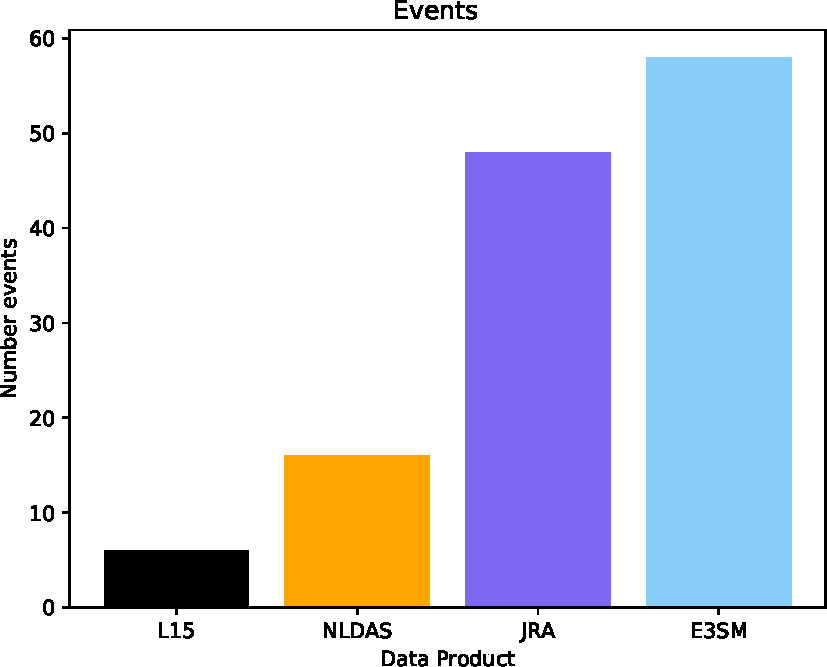
\includegraphics[width=0.442\linewidth]{{figs/cropped/events_AB}.pdf} & 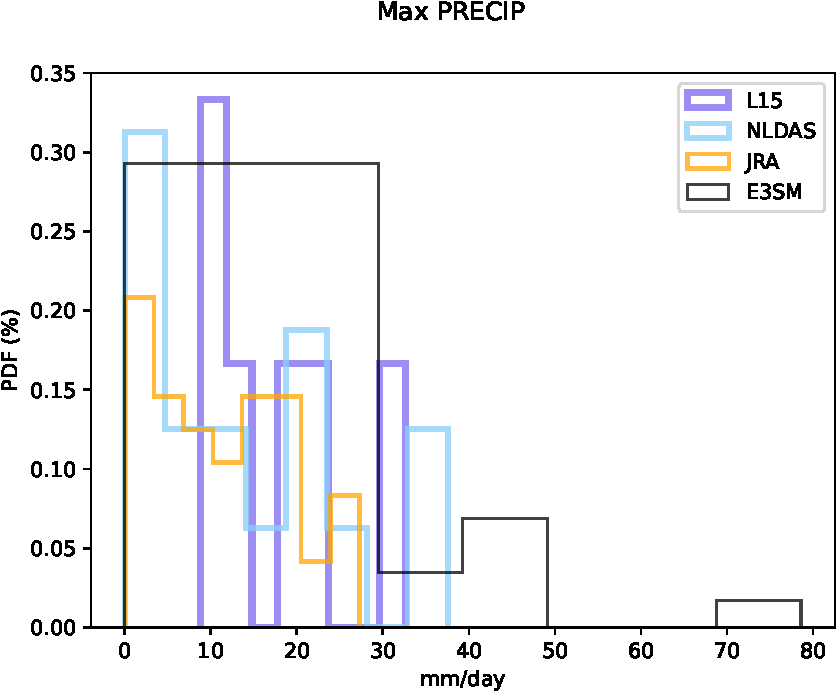
\includegraphics[width=0.451\linewidth]{{figs/cropped/Max_precip_AB}.pdf} \\
%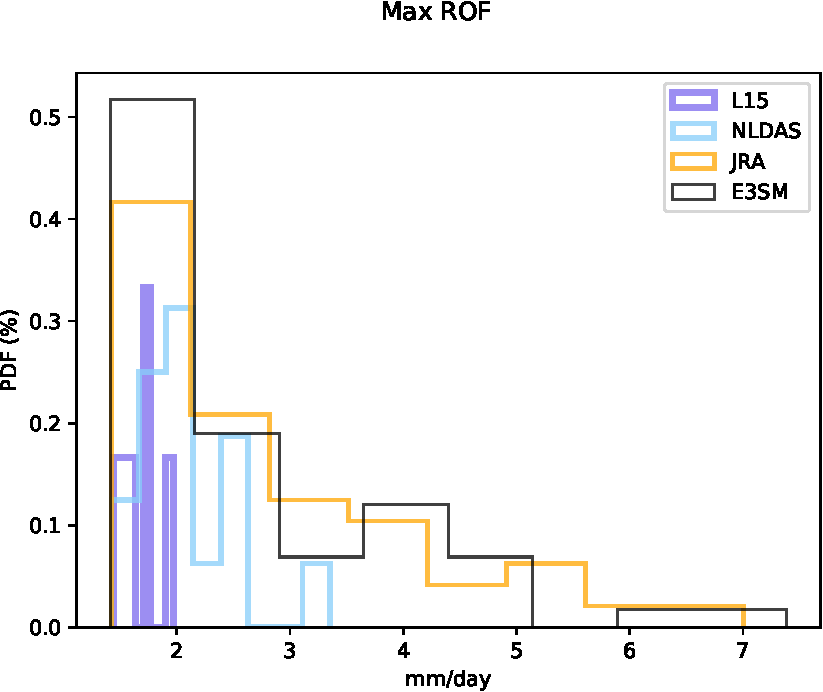
\includegraphics[width=0.451\linewidth]{{figs/cropped/Max_runoff_AB}.pdf} & 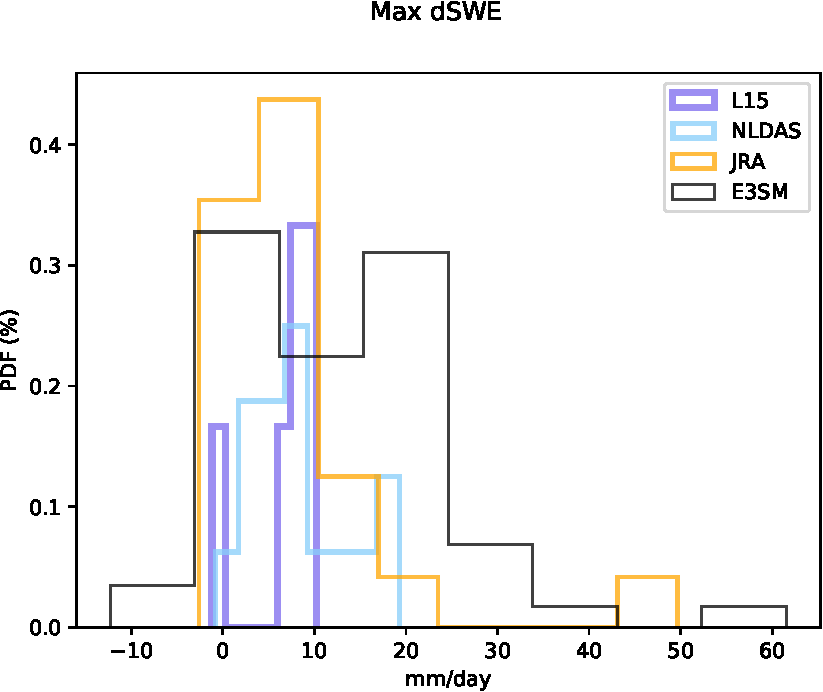
\includegraphics[width=0.451\linewidth]{{figs/cropped/Max_dSWE_AB}.pdf}
%\end{tabular}
%\caption{Histogram statistics for RoS events within the FIXED detection framework. The number of RoS events for each product from 1985-2005 is shown in the top left. The other three panels show frequency distributions of the daily rate (mm/day) of maximum precipitation (PRECIP), maximum runoff (ROF), and maximum change in SWE (dSWE, snowmelt positive).}
%\label{fig:histograms2}
%\end{figure}

\begin{figure}
\begin{tabular}{cc}
\begin{overpic}[width=0.45\linewidth]{{figs/cropped/events_AB}.pdf}
\put (11,72) {\contour{white}{\large a.}}
\end{overpic}
&
\begin{overpic}[width=0.45\linewidth]{{figs/cropped/Max_precip_AB}.pdf}
\put (11,72) {\contour{white}{\large b.}}
\end{overpic}
\vspace{0.10cm} \\
\begin{overpic}[width=0.45\linewidth]{{figs/cropped/Max_runoff_AB}.pdf}
\put (11,72) {\contour{white}{\large c.}}
\end{overpic}
&
\begin{overpic}[width=0.45\linewidth]{{figs/cropped/Max_dSWE_AB}.pdf}
\put (11,72) {\contour{white}{\large d.}}
\end{overpic}
\end{tabular}
\caption{Histogram statistics for RoS events within the FIXED detection framework. The number of RoS events for each product from 1985-2005 is shown in the top left. The other three panels show frequency distributions of the daily rate (mm/day) of maximum precipitation (PRECIP), maximum runoff (ROF), and maximum change in SWE (dSWE, snowmelt positive).}
\label{fig:histograms2}
\end{figure}

%\begin{figure}
%\begin{tabular}{cc}
%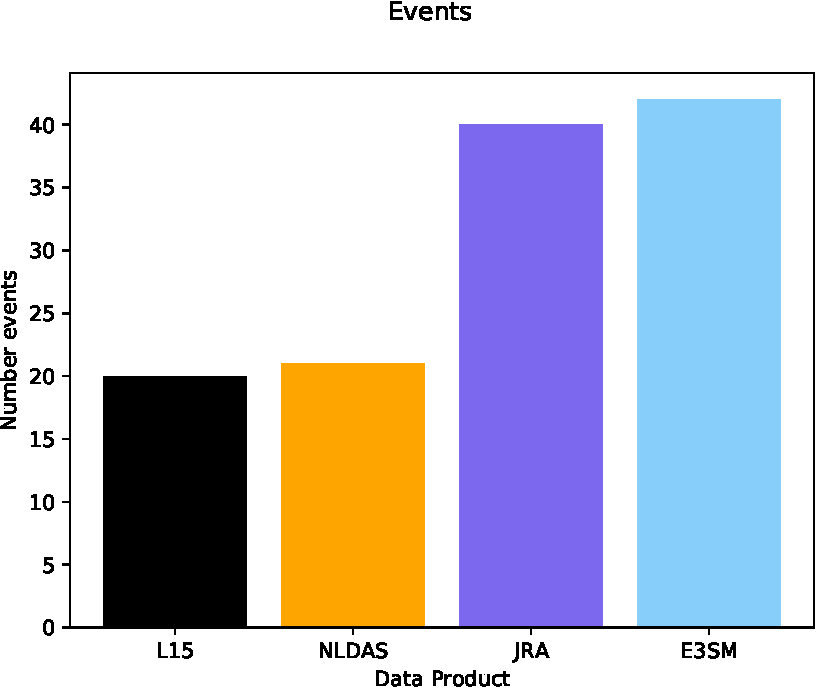
\includegraphics[width=0.442\linewidth]{{figs/cropped/events_95}.pdf} & 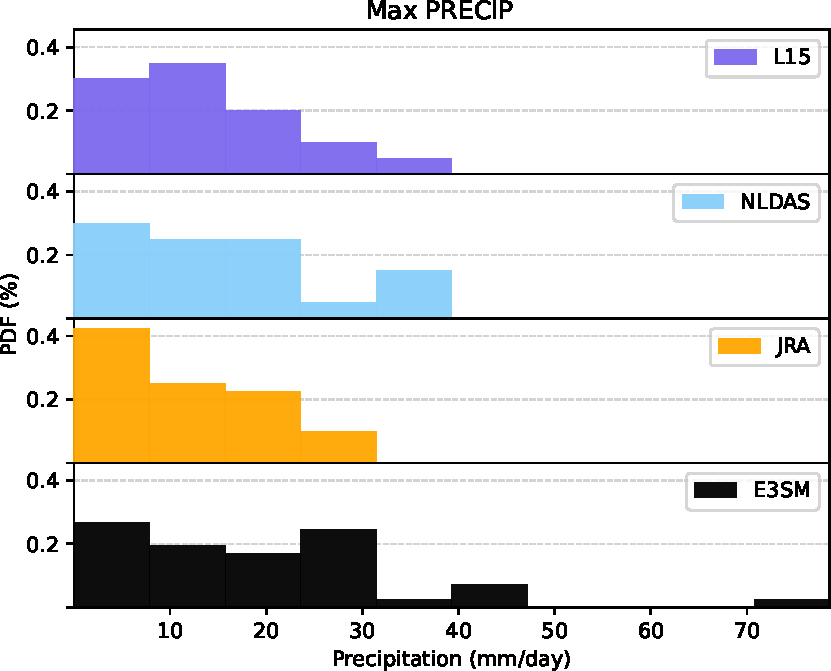
\includegraphics[width=0.451\linewidth]{{figs/cropped/Max_precip_95}.pdf} \\
%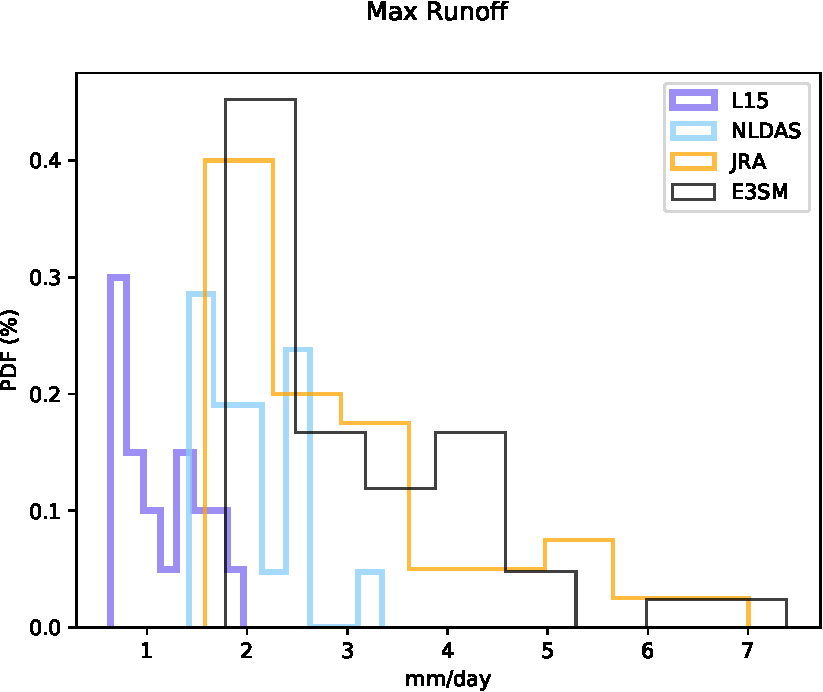
\includegraphics[width=0.451\linewidth]{{figs/cropped/Max_runoff_95}.pdf} & 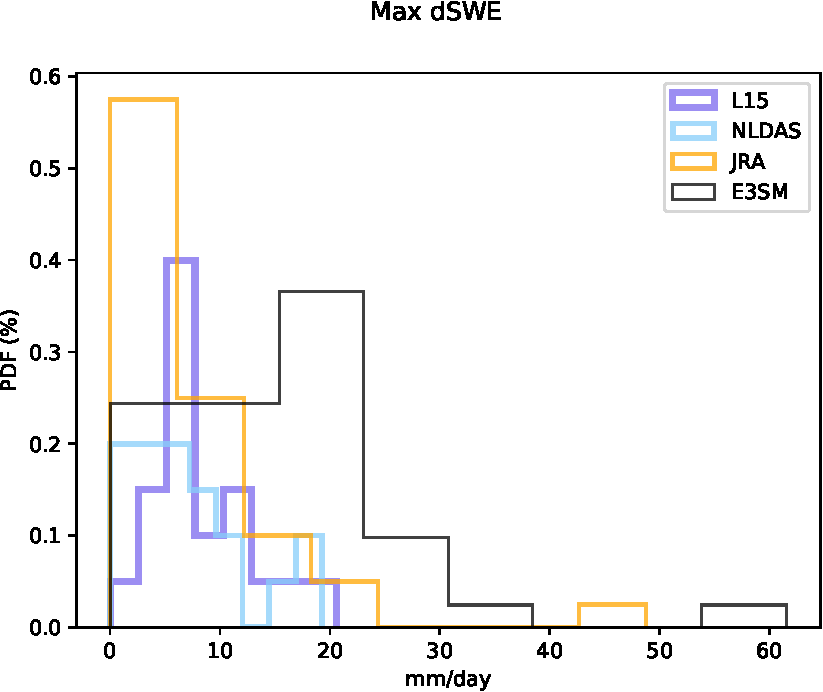
\includegraphics[width=0.451\linewidth]{{figs/cropped/Max_dSWE_95}.pdf}
%\end{tabular}
%\caption{Same as Fig. \ref{fig:histograms2} except for the RELATIVE detection thresholds.}
%\label{fig:histograms}
%\end{figure}

\begin{figure}
\begin{tabular}{cc}
\begin{overpic}[width=0.45\linewidth]{{figs/cropped/events_95}.pdf}
\put (11,72) {\contour{white}{\large a.}}
\end{overpic}
&
\begin{overpic}[width=0.45\linewidth]{{figs/cropped/Max_precip_95}.pdf}
\put (11,72) {\contour{white}{\large b.}}
\end{overpic}
\vspace{0.10cm} \\
\begin{overpic}[width=0.45\linewidth]{{figs/cropped/Max_runoff_95}.pdf}
\put (11,72) {\contour{white}{\large c.}}
\end{overpic}
&
\begin{overpic}[width=0.45\linewidth]{{figs/cropped/Max_dSWE_95}.pdf}
\put (11,72) {\contour{white}{\large d.}}
\end{overpic}
\end{tabular}
\caption{Same as Fig. \ref{fig:histograms2} except for the RELATIVE detection thresholds.}
\label{fig:histograms}
\end{figure}


\subsection{Single-year evaluation}

\begin{figure}
\begin{tabular}{cc}
\begin{overpic}[width=0.45\linewidth]{{figs/cropped/L15_1995_events}.pdf}
\put (11.5,40) {\contour{white}{\large a.}}
\end{overpic}
&
\begin{overpic}[width=0.45\linewidth]{{figs/cropped/NLDAS_1995_events}.pdf}
\put (11.5,40) {\contour{white}{\large b.}}
\end{overpic}
\vspace{0.10cm} \\
\begin{overpic}[width=0.45\linewidth]{{figs/cropped/JRA_1995_events}.pdf}
\put (11.5,40) {\contour{white}{\large c.}}
\end{overpic}
&
\begin{overpic}[width=0.45\linewidth]{{figs/cropped/E3SM_1995_events}.pdf}
\put (11.5,40) {\contour{white}{\large d.}}
\end{overpic}
\end{tabular}
\caption{Time series of daily precipitation (PRECIP; green), surface runoff (ROF; orange), and SWE loss (dSWE; pink) during WY95 for each of the four products. Vertical purple shading denotes periods flagged as an RoS event. At the top of each time series are colored bars that denote extreme values (greater than the 75th percentile) of observed USGS streamflow at Harrisburg, Pennsylvania, with very dark hues representing 99th percentile values over the 1980-2005 period.}
\label{fig:yr-timeseries-comp}
\end{figure}

\begin{figure}
\begin{tabular}{cc}
\begin{overpic}[width=0.45\linewidth]{{figs/cropped/L15_1995_scatplot}.pdf}
\put (12,63) {\contour{white}{\Large a.}}
\end{overpic}
&
\begin{overpic}[width=0.45\linewidth]{{figs/cropped/NLDAS_1995_scatplot}.pdf}
\put (12,63) {\contour{white}{\Large b.}}
\end{overpic}
\vspace{0.10cm} \\
\begin{overpic}[width=0.45\linewidth]{{figs/cropped/JRA_1995_scatplot}.pdf}
\put (12,63) {\contour{white}{\Large c.}}
\end{overpic}
&
\begin{overpic}[width=0.45\linewidth]{{figs/cropped/E3SM_1995_scatplot}.pdf}
\put (12,63) {\contour{white}{\Large d.}}
\end{overpic}

\end{tabular}
\caption{Bubble plots comparing precipitation (PRECIP; y-axis), SWE change (dSWE; x-axis), and surface runoff (size of bubble) for each of the four datasets during WY95. For each bubble, the values come from the same calendar day. Filled bubbles were flagged by the algorithm as an RoS event (purple shaded periods in Fig. \ref{fig:yr-timeseries-comp}).}
\label{fig:bubble-comp}
\end{figure}

% \begin{figure}
% \centering
% \begin{tabularx}{\textwidth}{XX}
% 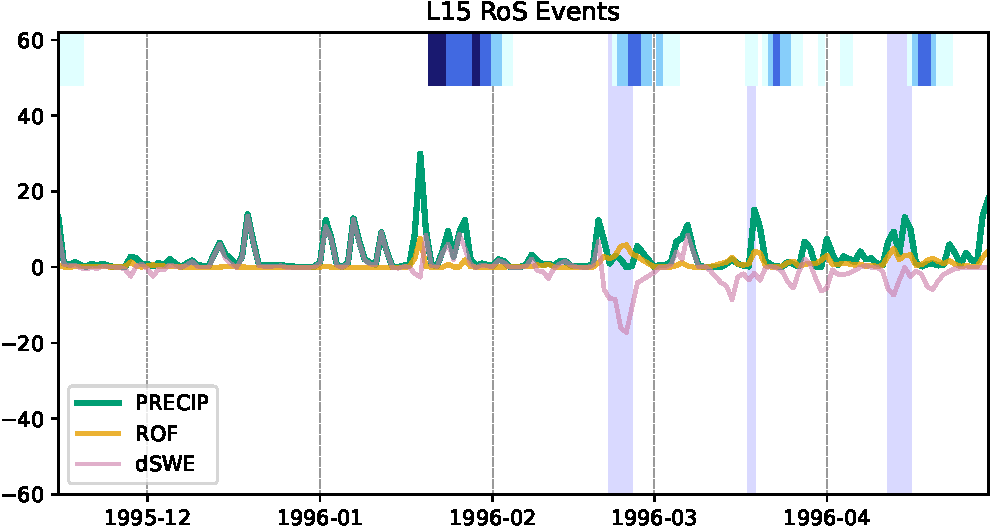
\includegraphics[width=1.0\linewidth]{{figs/cropped/L15_1995_events}.pdf} & 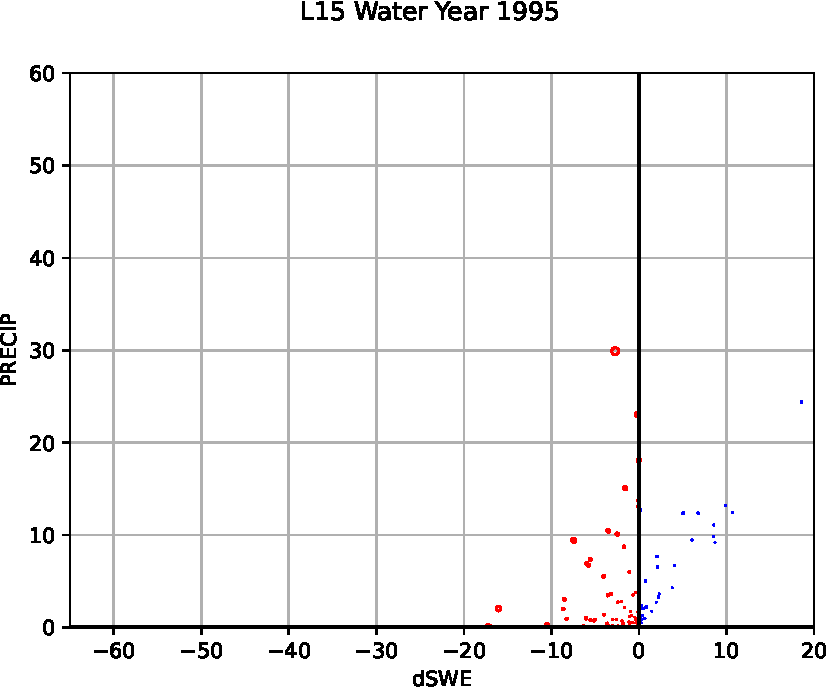
\includegraphics[width=0.75\linewidth]{{figs/cropped/L15_1995_scatplot}.pdf} \\ 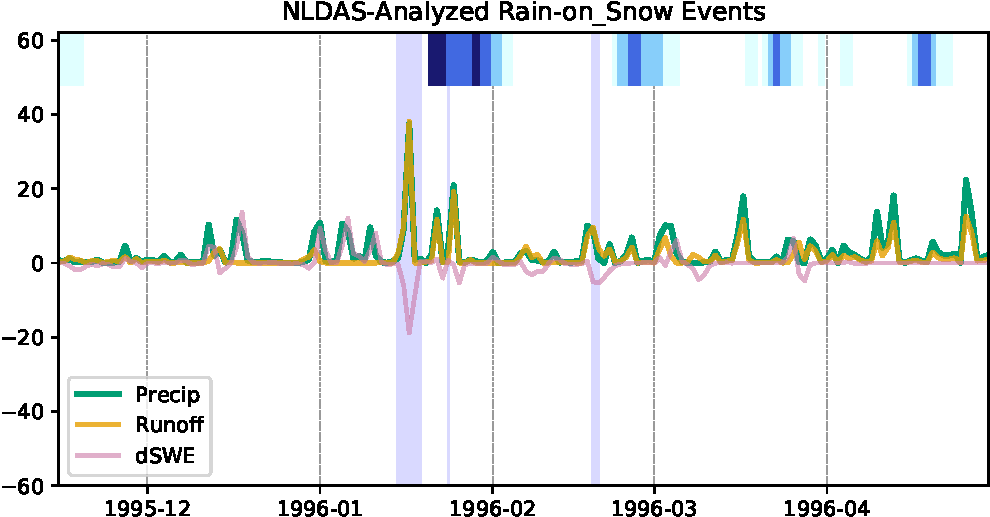
\includegraphics[width=1.0\linewidth]{{figs/cropped/NLDAS_1995_events}.pdf} & 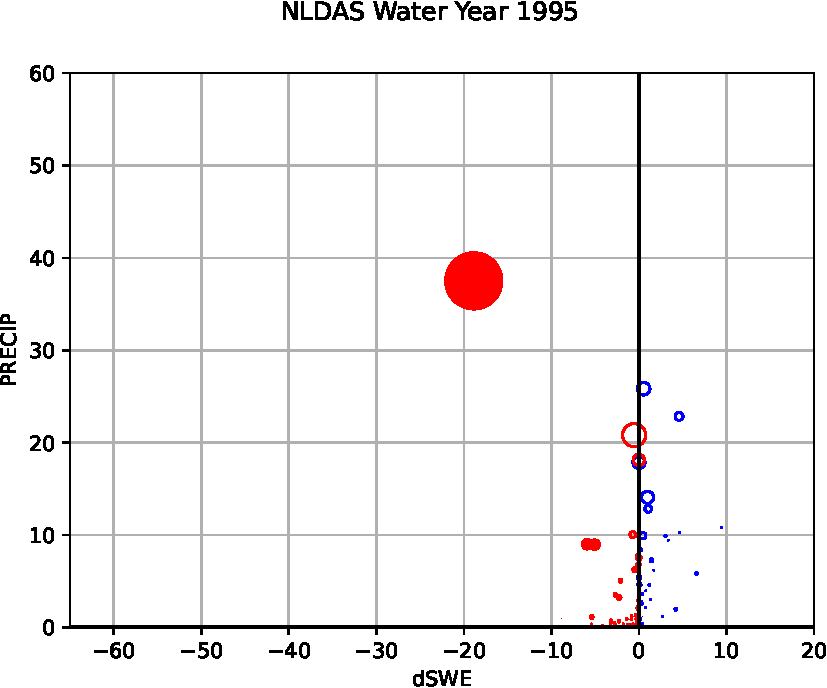
\includegraphics[width=0.75\linewidth]{{figs/cropped/NLDAS_1995_scatplot}.pdf} \\
%     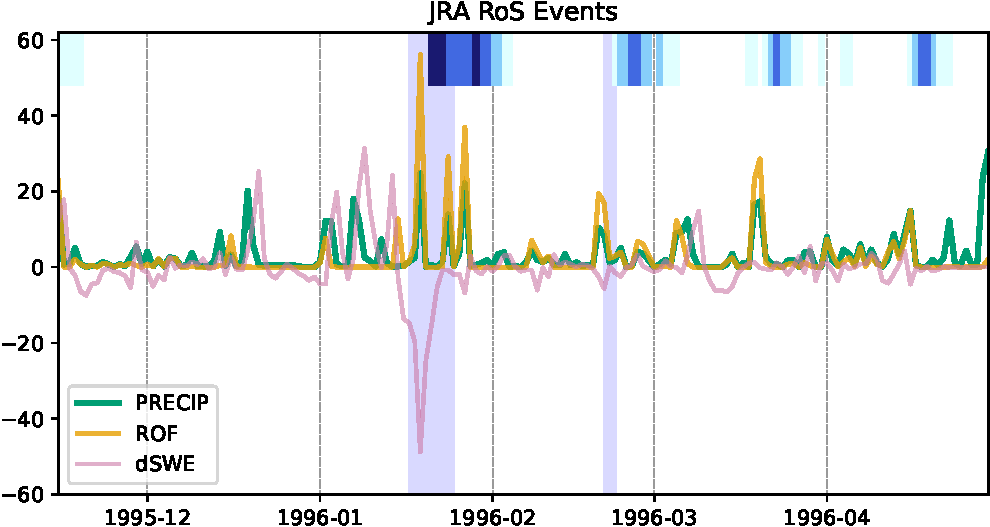
\includegraphics[width=1.0\linewidth]{{figs/cropped/JRA_1995_events}.pdf} & 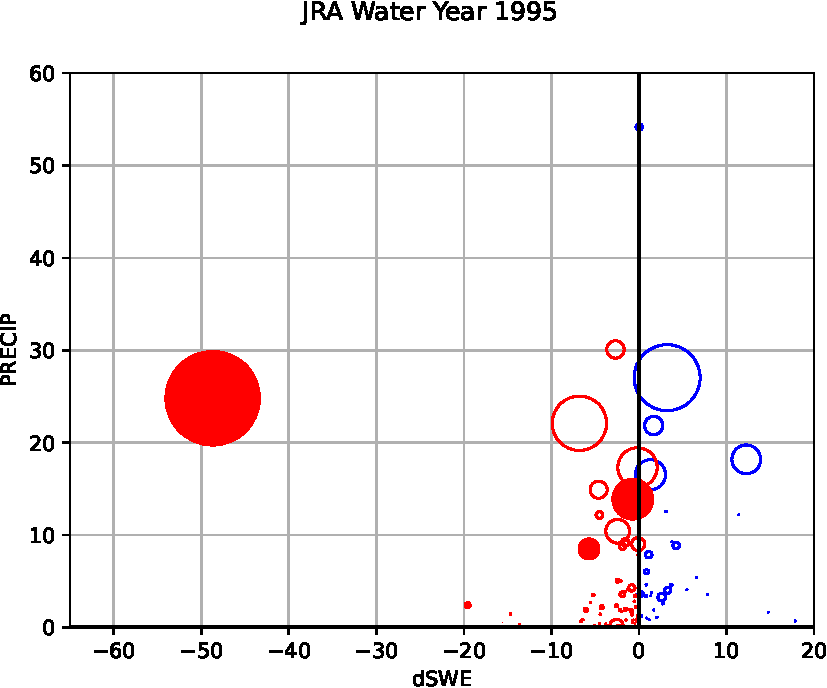
\includegraphics[width=0.75\linewidth]{{figs/cropped/JRA_1995_scatplot}.pdf} \\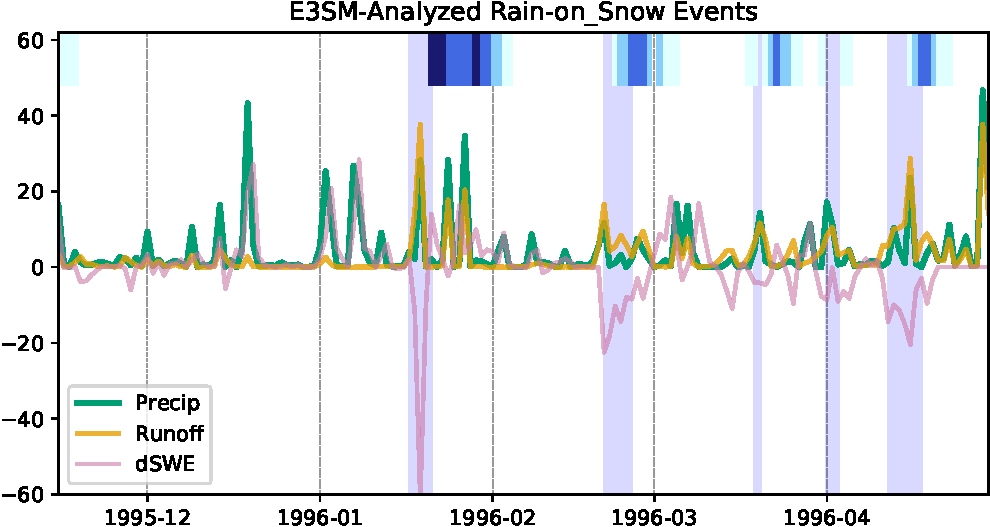
\includegraphics[width=1.0\linewidth]{{figs/cropped/E3SM_1995_events}.pdf} & 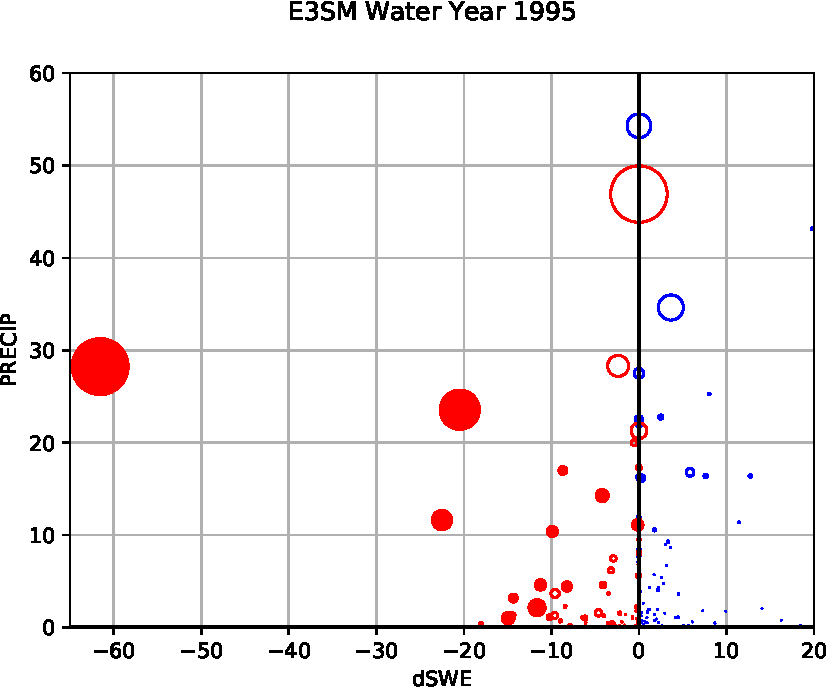
\includegraphics[width=0.75\linewidth]{{figs/cropped/E3SM_1995_scatplot}.pdf}
% \end{tabularx}
% \caption{(left) Time series of daily precipitation (PRECIP; green), surface runoff (ROF; orange), and change in SWE (dSWE; pink) during WY95 for each dataset. Vertical purple shading denotes periods flagged as a rain-on-snow (RoS) event using frameworks discussed in the Methods. Along the top x-axis of each time series is a colored bar series that denotes extreme values (greater than 75\%) of observed USGS streamflow at Harrisburg, PA with the darkest hues representing 99\% values over the 1980-2005 period. (right) Bubble plots comparing daily PRECIP (y-axis), dSWE (x-axis), and ROF (size of bubble) during WY95. Bubbles that are filled were days flagged by the RoS algorithm as occurring during an RoS event.}
% \label{fig:merged-wy}
% \end{figure}

To further explore RoS events at a more granular level we focus on results associated with the 1995 water year (WY95, October 1995 to September 1996).
We chose this WY since this includes the January 1996 SRB flood that is often used for disaster planning purposes in the region \citep{army2001non}.
The same visualizations for other WYs are included in the data download associated with this manuscript.

Figure \ref{fig:yr-timeseries-comp} shows the SRB daily WY95 time series of basin-integrated PRECIP, ROF, and dSWE.
Negative (positive) dSWE denotes snowmelt (accumulation).
Vertical shading denotes RoS events that were flagged by the algorithm (using the RELATIVE thresholds).
At the top of each panel is a stripe with four different shadings, representing days where streamflow exceeded the 75th, 90th, 95th, and 99th relative percentiles over the 1985-2005 period at the US Geological Survey (USGS) gage at Harrisburg, Pennsylvania (USGS \#01570500), with deepest blues representing highly anomalous flow conditions.

The January 17-18, 1996 event is readily apparent for three of the four data products (NLDAS, JRA, and E3SM).
Observed streamflow spiked during and immediately after the RoS event as shown by the dark blue stripes at the top of each time series, indicating a lag between when the RoS event algorithm identifies changes in PRECIP, dSWE, and ROF and the observed daily streamflow gage observation at Harrisburg (namely, the 99th percentile streamflow exceedance).
While this is operationally the largest RoS event observed over the period, there remain large discrepancies in the hydrometeorological conditions between the datasets.
The dSWE signal is the largest in magnitude within JRA and E3SM compared to NLDAS.
L15 shows a very minimal dSWE, to the point that $t_{\textrm{dSWE}}$ is not exceeded in the detection algorithm.
PRECIP is more similar across the three datasets, implying that the reduced ROF in L15 is likely due to minimal snowmelt.

All products also indicate a second, more moderate RoS event during the last third of February, although L15 and E3SM (JRA and E3SM) show larger dSWE (ROF) signals than the other two datasets.
The USGS gage streamflow also exceeded the 95th percentile for this RoS event.
More moderate flooding also appeared to occur in March and April although the detection algorithm only flagged such events in L15 and E3SM.
We also emphasize that all RoS events flagged by the detection algorithm resulted in well-above-average streamflow, highlighting the efficacy of the detection algorithm in capturing meaningful hydrometeorological extremes from basin-scale climate data.

Another way to visualize the WY95 RoS events is shown in Fig. \ref{fig:bubble-comp}.
This plot shows the daily distribution of all three hydrometeorological quantities that make up a RoS event by plotting dSWE on the x-axis, PRECIP on the y-axis, and the size of the x-y marker depicts the magnitude of ROF.
Markers are filled if the RoS event criteria are satisfied (RELATIVE) for that calendar day and are colored red (blue) if there is dSWE loss (gain).
The variability of the PRECIP (y-axis) is the most similar between the two ESMs, although all products include at least one day of precipitation greater than 30 mm when averaged over the SRB.
Larger differences across datasets are noted for the other two RoS event response variables.
JRA and E3SM produce a wider spread in both RoS and non-RoS events along the x-axis, indicating that the two ESMs produce days with the largest magnitudes of dSWE.
Further, L15 has markers that are small in size, indicating low daily ROF magnitudes when compared to the other three products.
There is a substantial spread across the four datasets, even over comparable time series with well-defined and record-setting RoS events.
This is likely due to daily differences in the timing of storms, the amount of water vapor transport and precipitation they produce, and how close surface air temperatures are to freezing conditions that in turn influence if a meteorological event leads to an increase in snow accumulation or results in an RoS event.

\subsection{Evaluation of a single event}

%\begin{figure}
%\noindent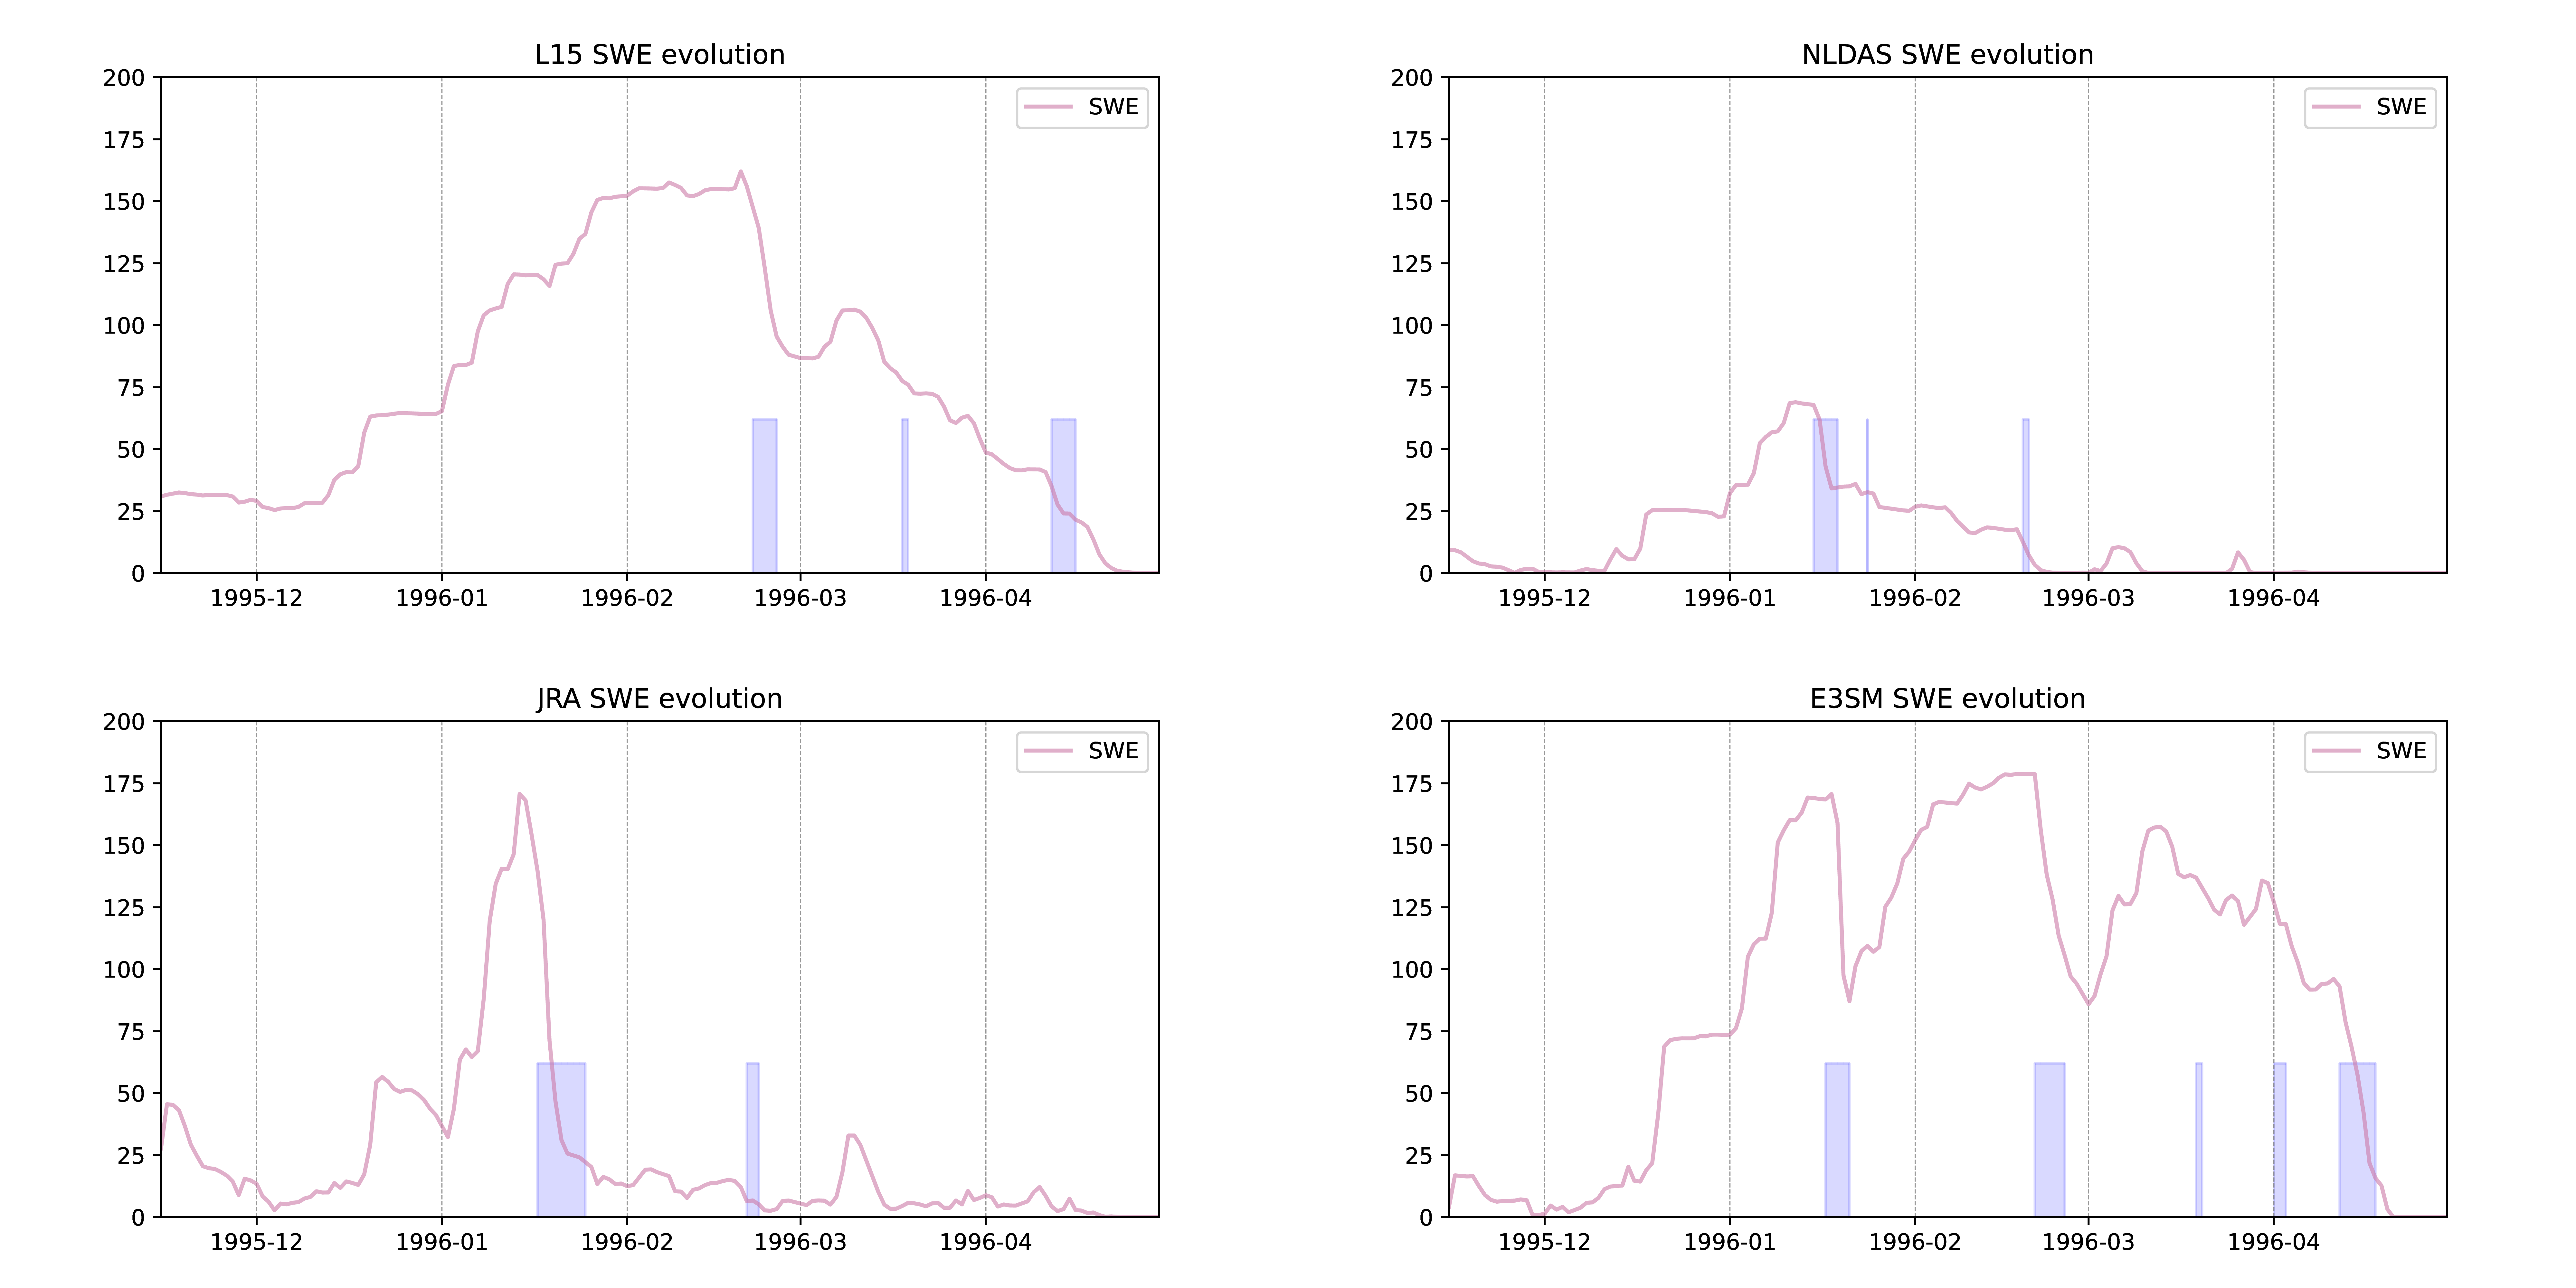
\includegraphics[width=0.95\textwidth]{figs/cropped/merged_SWE_1995.png}
%\caption{Daily SWE timeseries averaged over the SRB during WY95 for all four data products. Shaded in blue are the same events from Fig. \ref{fig:yr-timeseries-comp}.}
%\label{fig:allswewy95}
%\end{figure}

%\begin{figure}
%\begin{tabular}{cc}
%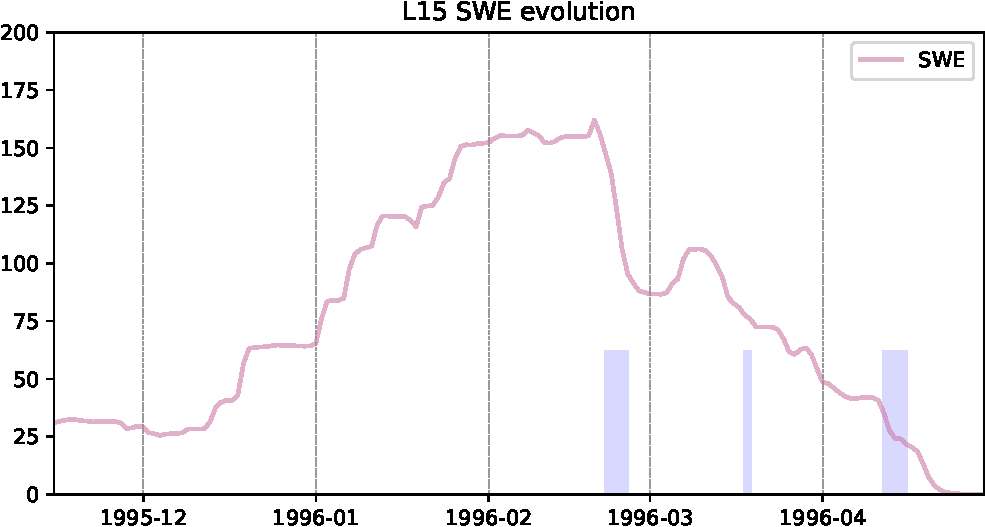
\includegraphics[width=0.45\linewidth]{{figs/cropped/L15_1995_SWE}.pdf} & 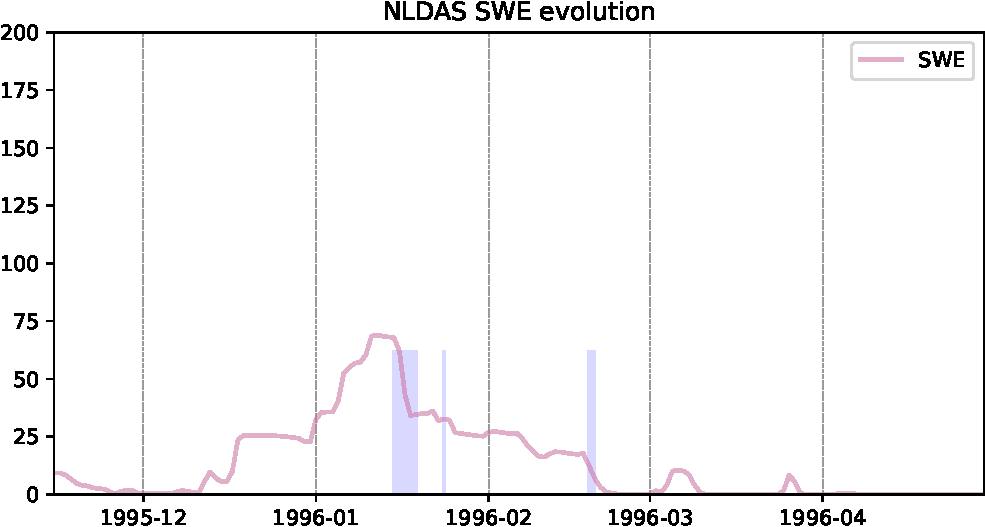
\includegraphics[width=0.45\linewidth]{{figs/cropped/NLDAS_1995_SWE}.pdf} \\
%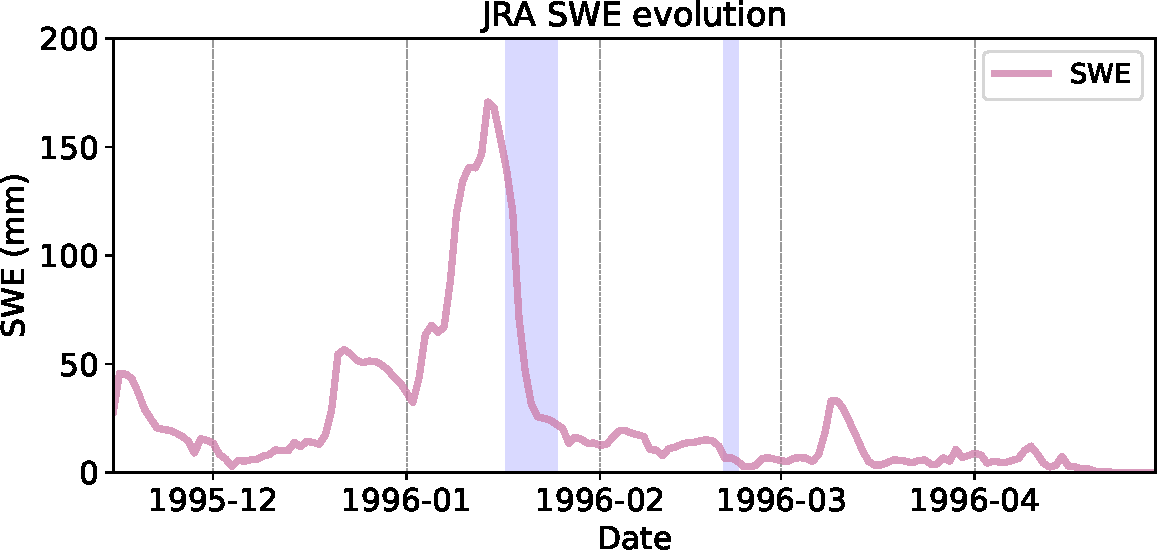
\includegraphics[width=0.45\linewidth]{{figs/cropped/JRA_1995_SWE}.pdf} & 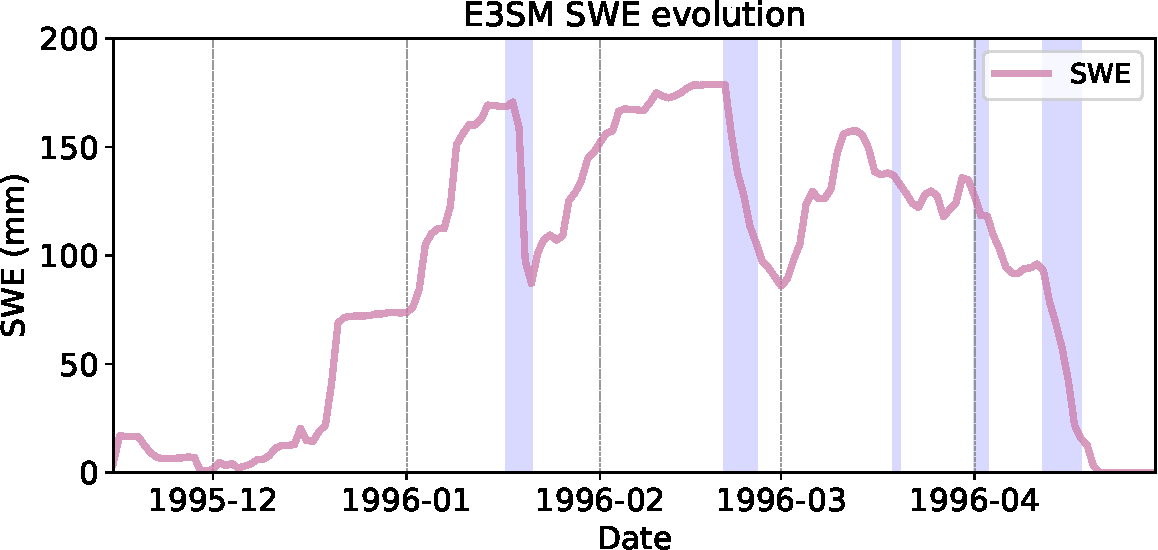
\includegraphics[width=0.45\linewidth]{{figs/cropped/E3SM_1995_SWE}.pdf}
%\end{tabular}
%\caption{Daily SWE timeseries averaged over the SRB during WY95 for all four data products. Shaded in blue are the same events from Fig. \ref{fig:yr-timeseries-comp}.}
%\label{fig:allswewy95}
%\end{figure}

%%% \put HORIZ, VERT from bottom left
\begin{figure}
\begin{tabular}{cc}
\begin{overpic}[width=0.45\linewidth]{{figs/cropped/L15_1995_SWE}.pdf}
\put (11,39.5) {\contour{white}{\large a.}}
\end{overpic}
&
\begin{overpic}[width=0.45\linewidth]{{figs/cropped/NLDAS_1995_SWE}.pdf}
\put (11,39.5) {\contour{white}{\large b.}}
\end{overpic}
\vspace{0.10cm} \\
\begin{overpic}[width=0.45\linewidth]{{figs/cropped/JRA_1995_SWE}.pdf}
\put (11,39.5) {\contour{white}{\large c.}}
\end{overpic}
&
\begin{overpic}[width=0.45\linewidth]{{figs/cropped/E3SM_1995_SWE}.pdf}
\put (11,39.5) {\contour{white}{\large d.}}
\end{overpic}
\end{tabular}
\caption{Daily SWE timeseries averaged over the SRB during WY95 for all four data products. Shaded in blue are the same events from Fig. \ref{fig:yr-timeseries-comp}.}
\label{fig:allswewy95}
\end{figure}

% \begin{figure}
% \begin{tabular}{cc}
% 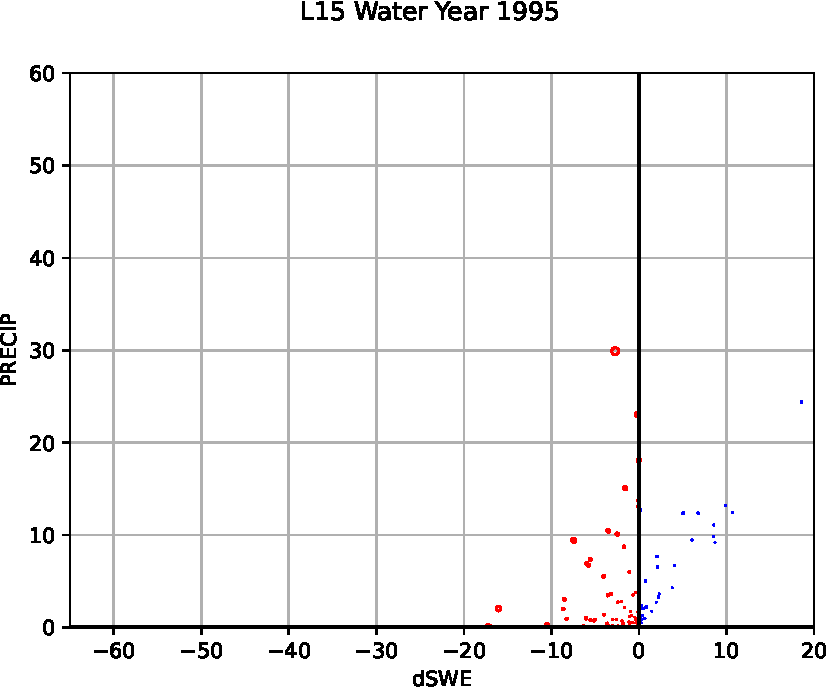
\includegraphics[width=0.45\linewidth]{{figs/cropped/L15_1995_scatplot}.pdf} & 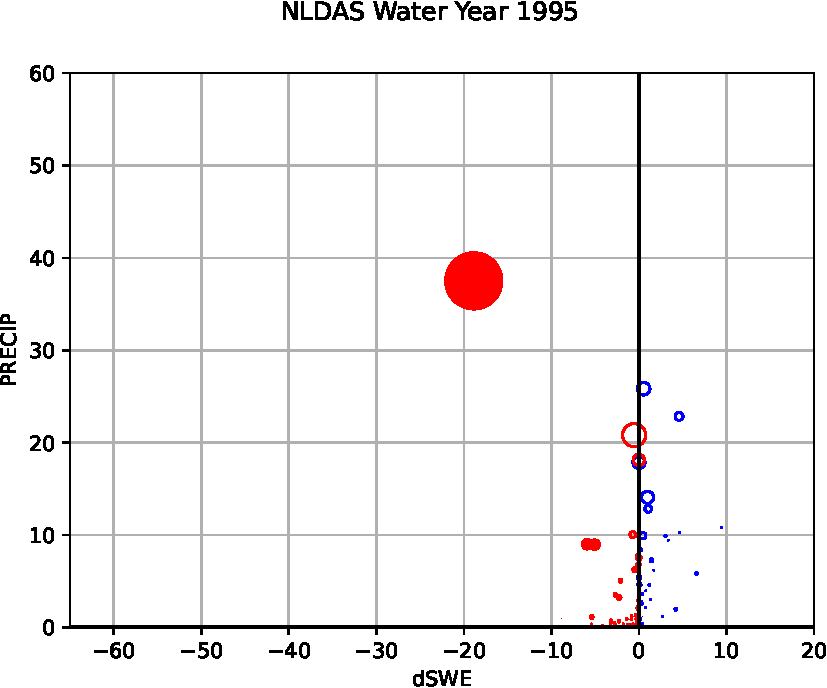
\includegraphics[width=0.45\linewidth]{{figs/cropped/NLDAS_1995_scatplot}.pdf} \\
% 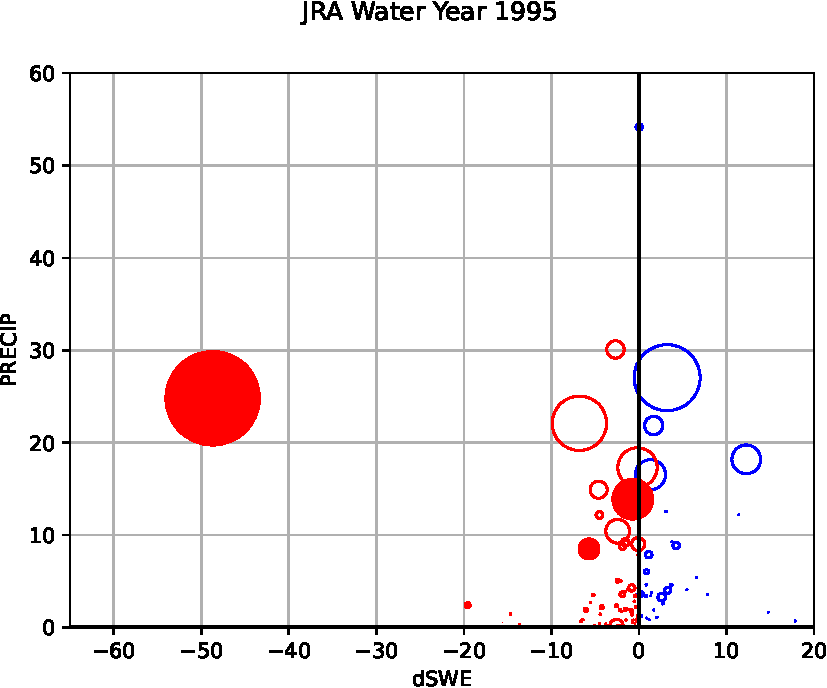
\includegraphics[width=0.45\linewidth]{{figs/cropped/JRA_1995_scatplot}.pdf} & 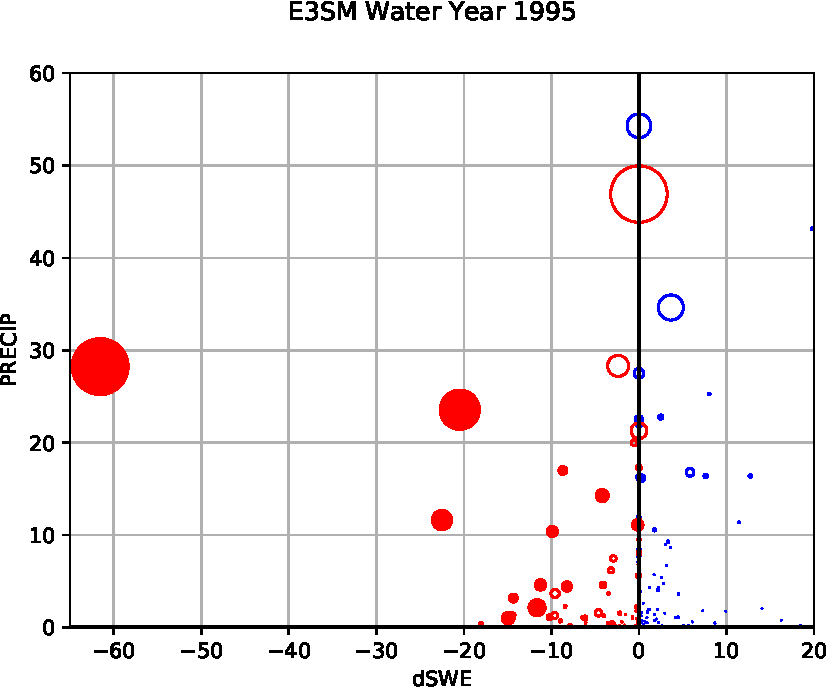
\includegraphics[width=0.45\linewidth]{{figs/cropped/E3SM_1995_scatplot}.pdf}
% \end{tabular}
% \caption{....}
% \label{fig:allswewy95}
% \end{figure}

One notable question given the above analysis (Fig. \ref{fig:yr-timeseries-comp}) is why the January 1996 event is captured differently across the products, particularly `why is it `unseen' by the L15 dataset?'
Fig. \ref{fig:allswewy95} shows the SRB evolution of total on-surface SWE over WY95 for all datasets.
All products show increasing SWE from mid-December onwards, albeit with varying accumulation rates and maximum depths.
The datasets most differ in the SWE ablation during mid-January, with L15 (Fig. \ref{fig:allswewy95}a) showing essentially no ablation of the existing snowpack, JRA (Fig. \ref{fig:allswewy95}c) showing near total ablation, and NLDAS and E3SM (Fig. \ref{fig:allswewy95}b,d) lying somewhere between the two extremes.

To untangle the potential source of this discrepancy, Fig. \ref{fig:1996eventtrace} shows the temperature (red line, right axis) at the grid cell nearest Harrisburg for the four products during the 1996 event.
Also included is the temperature trace observed at Harrisburg (thin gold line) as recorded in National Oceanic and Atmospheric (NOAA) surface weather station archives along with a reference freezing line (black). The surface relative humidity is indicated by the dashed purple line (right axis) and the product-specific associated precipitation rate (mm/hr) partitioned into rain (green) and snow (cyan) is denoted by bars (left axis).

%https://journals.ametsoc.org/view/journals/clim/26/23/jcli-d-12-00508.1.xml
%http://livnehpublicstorage.colorado.edu:81/Livneh.2013.CONUS.Dataset/

\begin{figure}
\begin{overpic}[width=0.8\textwidth]{figs/cropped/precip_vs_t_1996.pdf}
\put (7,65) {\contour{white}{\Large a.}}
\put (48.5,65) {\contour{white}{\Large b.}}
\put (7,34.25) {\contour{white}{\Large c.}}
\put (48.5,34.25) {\contour{white}{\Large d.}}
\end{overpic}
\caption{Evolution of reference height surface air temperature, relative humidity, and precipitation during the January 1996 SRB RoS flood event across data products. Data is taken from the grid cell nearest to Harrisburg, Pennsylvania. The left axis corresponds to the precipitation rate (shown in bars from the bottom) reported by the product. Green bars indicate rainfall (precipitation occurring when $T_s > 0$\degree{}C) and cyan bars indicate snowfall (precipitation occurring when $T_s <= 0$\degree{}C). The right axes show reference height surface air temperature as denoted by the solid red line, and relative humidity as denoted by the purple dashed line. A thick black horizontal line indicates 0\degree{}C air temperature (273.15 K). The thin gold line on each panel represents the observed temperature trace at Harrisburg over the period.}
\label{fig:1996eventtrace}
\end{figure}

None of the four products precisely match the observed temperature, although we acknowledge that this is, at least, partly due to the spatial resolution of the data.
While the timing of the temperature increase associated with the warm air advection component of the event is well matched in NLDAS (Fig. \ref{fig:allswewy95}b) and E3SM (Fig. \ref{fig:allswewy95}d), both products have a slight cool bias.
The overall temperature maximum is better matched by JRA (Fig. \ref{fig:allswewy95}c), although the peak occurs approximately 6 hours earlier than in observations. An opposite shift is seen in L15 data, with the observed temperature peak leading L15's temperature peak by approximately 6 hours (Fig. \ref{fig:allswewy95}a).

Across all four datasets, only L15 reports below-freezing temperatures between January 18th at 12Z and January 19th at 18Z.
This occurs because L15 only leverages daily minimum and maximum observed temperatures to construct temperature fields.
At each L15 grid cell, temperature minima and maxima are assumed to occur at sunrise and approximately late afternoon, respectively, with an interpolation spline used to provide information at intermediate hours \citep{bohn2013global}.
These temperatures are always assumed to occur on the day of record \citep{livneh2015spatially}, which is relevant because the actual temperature minimum on January 19th occurred during the local afternoon after the passage of a cold front \citep{leathers1998severe}.
A similar, regular cycle is seen in the L15 relative humidity, with near-saturated surface conditions only occurring for approximately 3-hour windows each day. The other three data products show the increased moisture advection ahead of the precipitation maximum, with near-saturated surface air mass for large periods of the 72 hours preceding the initiation of the flood event.
Therefore, for this event, the diurnal cycle of thermodynamic variables is more strongly influenced by atmospheric dynamics than solar insolation.
We emphasize that this timing is actually quite important since factors such as temperature and surface humidity (and associated sensible and latent heat fluxes) are typically dominant drivers of snow ablation in high snowmelt events \citep{mazurkiewicz2008assessing,wurzer2016influence,harpold2018humidity} and need to line up concurrently to produce compound extremes like the one observed in 1996.

To understand how this could impact snowpack metamorphism, we also investigate precipitation during the event.
We can assume precipitation type at the surface is determined by whether the reference height surface air temperature is above or below freezing, which is the manner in which the majority of land surface models partition precipitation \citep{harpold2017rain,jennings2018spatial,Woodburn2021}.
Since L15 contains below-freezing temperatures between 00Z and 12Z on January 19, it is the only product that partitions a fraction of precipitation into the frozen state during the peak of the event.
Further, since daily precipitation is evenly partitioned into sub-daily bins to force VIC, L15 registers more precipitation during this period than the other products (which typically peak after 12Z on January 19).

We argue this motivates the following interpretation.
In L15, snowpack lost due to melt during the above-freezing temperatures during the 1996 event is, at least, partially offset by new snow on the ground that falls during the event due to below-freezing temperatures.
These below-freezing periods and reduced relative humidity at the surface also mitigate any snowmelt in the land surface model that would be associated with enthalpy fluxes (either sensible or latent heat) into the existing snowpack.
When combined, this explains the lack of a decline in L15 SWE and subsequent large spike in ROF in Fig. \ref{fig:yr-timeseries-comp}.
All other datasets show a more prolonged period of above-freezing temperatures with high specific humidity during the window noted above, with nearly all precipitation during this period falling as rain versus snow.
This induced varying degrees of snowmelt in E3SM, NLDAS, and JRA that are sufficient to trigger the RoS detection algorithm.

\conclusions

We interrogate four different gridded climate data products that include PRECIP, ROF, and SWE in order to quantify differences in the representation of coupled land-atmosphere processes that lead to flooding events in the historical record.
In particular, we focus on RoS floods over the SRB and devise an algorithm for the automatic detection of RoS events that can be applied to any gridded dataset with relevant variables.

A detection algorithm flagging for times of collocated ROF and dSWE is generally successful at marking periods that will be followed by above-normal streamflow as measured by a gage in the basin.
We find using fixed thresholds for RoS-relevant variables applied uniformly across multiple gridded datasets leads to large discrepancies in event frequency over the historical period, up to a factor of 10.

Normalizing these thresholds by each dataset's climatology (relative thresholds based on daily percentiles) improves agreement.
However, there remains approximately a factor of two difference between event counts, implying that the underlying distributions are fundamentally different in both shape and magnitude across the data analyzed.

% Notably, although we refer to automated algorithm-flagged events as RoS events, there is no explicit PRECIP threshold.
% With that said, we find that 75\% of automated algorithm-flagged events have at least one day of $>5$ mm/day of basin-averaged precipitation and 95\% have at least one day of measurable precipitation ($>$1 mm/day).
% This implies that while ablation-only snowmelt events can lead to flooding, the vast majority of events producing large flood signals involve some form of precipitation as well.

%A common misconception is that RoS events are generated by warm rain transferring heat to the snowpack which then ripens or ablates it.

This underscores the complex assessment of such flood events -- even products representing the historical record contain a large spread in hydrometeorological quantities provided to end users. The spatiotemporal dependencies of how meteorological data is generated for land surface and/or hydrological model forcing are critically important.
While spatial resolution of data is important, particularly for snow processes in complex terrain \citep{henn2018an,Woodburn2021}, we show that the time resolution of data used to derive surface water conditions is just as critical for transient extremes, such as RoS events.
This is because the timing of synoptic variations in reference height surface air temperature and humidity that dictate snowmelt and precipitation phase can occur on the order of hours at local scales and can have an outsized role in compound extreme event representation if those variations are threshold-dependent (e.g., storm rain-snow partitioning and alterations to the freezing line at the land surface).

Since RoS events in regions of ephemeral snow (e.g., SRB) can have rapid changes in surface forcing at hourly timescales (e.g., \citet{leathers1998severe}), temporally coarse data applied to force LSMs may result in an underprediction of RoS frequency.
This may occur if time-interpolated data (and/or less frequent coupling) smooths and/or clips out short-term extrema and results in mismatched forcing or reduced day-to-day variability of multiple, co-dependent anomalies (e.g., temperature and precipitation extremes) required to accurately simulate historical, decision-relevant hydrometeorological extremes (e.g., 1996 SRB RoS event). We note that this effect can be independent of the model timestep itself. For example, the L15 data disaggregates precipitation data across sub-daily timesteps and uses a diurnal spline to reconstruct near-surface atmospheric conditions. While the LSM used is integrated at smaller timescales, the effective time resolution of the forcing data remains daily.

We also show that even though a dataset is provided at much coarser spatial resolutions than is desired (e.g., JRA and E3SM), model-derived datasets that are more frequently coupled and/or constrained at shorter timescales (e.g., reanalysis products and nudged ESMs) may produce more accurate land-atmosphere interactions and better representation of decision-relevant hydrometeorological extremes, particularly at basin (and larger) spatial scales. However, these products will likely suffer in the spatial representation of hydrometeorology in regions of high heterogeneity.

We want to emphasize that this work doesn't aim to suggest a `superior' dataset writ large. For example, even though L15 does not capture the 1996 SRB flood as well as other products here, it has been an invaluable tool for studying climate extremes such as heat waves \citep{mazdiyasni2015substantial}, droughts \citep{pendergrass2020flash,williams2020large}, and wildfires \citep{williams2019observed} (amongst others) in the US.
Rather, we offer a few suggestions about leveraging hydrometeorological data for application purposes.
It is recommended that gridded climate data developers consider the temporal resolution of land surface forcing if the representation of daily (or sub-daily) hydrometeorological extrema is desirable, particularly from a use-inspired or decision-relevant context \citep{Jagannathan2021}.
While we do not downscale any datasets in this study, it is likely that using different meteorological data to force the same land surface and/or hydrological model will result in vastly different predicted streamflows, particularly for RoS events when variables are spatiotemporally co-dependent and would be sensitive to any post-processing adjustments (e.g., mean climatological correction). When possible, sub-daily information about atmospheric conditions should be included in meteorological forcing data.

From a stakeholder perspective, this is an important consideration when back-testing models, and, in particular, applying such models to evaluate tail risks (e.g., 1-in-100-year flood events and how they may change in a future climate).
The results here show longer tails in the fully-coupled ESM-derived climate data, which may impact return rates of extreme events, even if calibrated or bias-corrected after the fact.
Therefore, care must be taken when applying data requiring coupling between the atmosphere and land surface (and riverine) components, whether generated dynamically or statistically.
While post-processing adjustments to the mean climatology may be desirable, these adjustments can alter decision-relevant hydrometeorological extremes that reside in the tail of the distribution.



%%

%  Numbered lines in equations:
%  To add line numbers to lines in equations,
%  \begin{linenomath*}
%  \begin{equation}
%  \end{equation}
%  \end{linenomath*}



%% Enter Figures and Tables near as possible to where they are first mentioned:
%
% DO NOT USE \psfrag or \subfigure commands.
%
% Figure captions go below the figure.
% Table titles go above tables;  other caption information
%  should be placed in last line of the table, using
% \multicolumn2l{$^a$ This is a table note.}
%
%----------------
% EXAMPLE FIGURES
%
% \begin{figure}
% \includegraphics{example.png}
% \caption{caption}
% \end{figure}
%
% Giving latex a width will help it to scale the figure properly. A simple trick is to use \textwidth. Try this if large figures run off the side of the page.
% \begin{figure}
% \noindent\includegraphics[width=\textwidth]{anothersample.png}
%\caption{caption}
%\label{pngfiguresample}
%\end{figure}
%
%
% If you get an error about an unknown bounding box, try specifying the width and height of the figure with the natwidth and natheight options. This is common when trying to add a PDF figure without pdflatex.
% \begin{figure}
% \noindent\includegraphics[natwidth=800px,natheight=600px]{samplefigure.pdf}
%\caption{caption}
%\label{pdffiguresample}
%\end{figure}
%
%
% PDFLatex does not seem to be able to process EPS figures. You may want to try the epstopdf package.
%

%
% ---------------
% EXAMPLE TABLE
%
% \begin{table}
% \caption{Time of the Transition Between Phase 1 and Phase 2$^{a}$}
% \centering
% \begin{tabular}{l c}
% \hline
%  Run  & Time (min)  \\
% \hline
%   $l1$  & 260   \\
%   $l2$  & 300   \\
%   $l3$  & 340   \\
%   $h1$  & 270   \\
%   $h2$  & 250   \\
%   $h3$  & 380   \\
%   $r1$  & 370   \\
%   $r2$  & 390   \\
% \hline
% \multicolumn{2}{l}{$^{a}$Footnote text here.}
% \end{tabular}
% \end{table}

%% SIDEWAYS FIGURE and TABLE
% AGU prefers the use of {sidewaystable} over {landscapetable} as it causes fewer problems.
%
% \begin{sidewaysfigure}
% \includegraphics[width=20pc]{figsamp}
% \caption{caption here}
% \label{newfig}
% \end{sidewaysfigure}
%
%  \begin{sidewaystable}
%  \caption{Caption here}
% \label{tab:signif_gap_clos}
%  \begin{tabular}{ccc}
% one&two&three\\
% four&five&six
%  \end{tabular}
%  \end{sidewaystable}

%% If using numbered lines, please surround equations with \begin{linenomath*}...\end{linenomath*}
%\begin{linenomath*}
%\begin{equation}
%y|{f} \sim g(m, \sigma),
%\end{equation}
%\end{linenomath*}

%%% End of body of article

%%%%%%%%%%%%%%%%%%%%%%%%%%%%%%%%
%% Optional Appendix goes here
%
% The \appendix command resets counters and redefines section heads
%
% After typing \appendix
%
%\section{Here Is Appendix Title}
% will show
% A: Here Is Appendix Title
%
%\appendix
%\section{Here is a sample appendix}

%%%%%%%%%%%%%%%%%%%%%%%%%%%%%%%%%%%%%%%%%%%%%%%%%%%%%%%%%%%%%%%%
%
% Optional Glossary, Notation or Acronym section goes here:
%
%%%%%%%%%%%%%%
% Glossary is only allowed in Reviews of Geophysics
%  \begin{glossary}
%  \term{Term}
%   Term Definition here
%  \term{Term}
%   Term Definition here
%  \term{Term}
%   Term Definition here
%  \end{glossary}

%
%%%%%%%%%%%%%%
% Acronyms
%   \begin{acronyms}
%   \acro{Acronym}
%   Definition here
%   \acro{EMOS}
%   Ensemble model output statistics
%   \acro{ECMWF}
%   Centre for Medium-Range Weather Forecasts
%   \end{acronyms}

%
%%%%%%%%%%%%%%
% Notation
%   \begin{notation}
%   \notation{$a+b$} Notation Definition here
%   \notation{$e=mc^2$}
%   Equation in German-born physicist Albert Einstein's theory of special
%  relativity that showed that the increased relativistic mass ($m$) of a
%  body comes from the energy of motion of the body—that is, its kinetic
%  energy ($E$)—divided by the speed of light squared ($c^2$).
%   \end{notation}


\codedataavailability{
L15 data was downloaded from the NOAA Administration Physical Science Laboratory, available at \url{https://psl.noaa.gov/data/gridded/data.livneh.html}. NLDAS-VIC4.0.5 data was downloaded from the NOAA National Centers for Environmental Prediction, available at \url{ftp://ldas.ncep.noaa.gov/nldas2/retrospective/vic4.0.5}. JRA-55 data was downloaded from the Research Data Archive at the National Center for Atmospheric Research, Computational and Information Systems Laboratory, available at \url{https://doi.org/10.5065/D6HH6H41}. The version of E3SM run here was v2.0.0-alpha.2-1816-gf9cbe57a2 and is available at https://github.com/E3SM-Project/E3SM. ERA5 data used to nudge the E3SM solution was downloaded from the Copernicus Climate Data Store (CDS), available at \url{https://www.ecmwf.int/en/forecasts/datasets/reanalysis-datasets/era5}. Station data for Harrisburg, PA was acquired from the Iowa Environmental Mesonet at \url{https://mesonet.agron.iastate.edu/}. The SRB is defined using a shapefile provided by the SRB Commission (\url{https://www.srbc.net/portals/susquehanna-atlas/data-and-maps/subbasins/index.html}). All processed data, figures, and scripts used to generate the results contained in this manuscript (along with README documentation) are archived at Zenodo and can be accessed at \url{https://doi.org/10.5281/zenodo.10412332}.
}


%%%%%%%%%%%%%%%%%%%%%%%%%%%%%%%%%%%%%%%%%%%%%%%%%%%%%%%%%%%%%%%%
%
%  ACKNOWLEDGMENTS
%
% The acknowledgments must list:
%
% >>>>	A statement that indicates to the reader where the data
% 	supporting the conclusions can be obtained (for example, in the
% 	references, tables, supporting information, and other databases).
%
% 	All funding sources related to this work from all authors
%
% 	Any real or perceived financial conflicts of interests for any
%	author
%
% 	Other affiliations for any author that may be perceived as
% 	having a conflict of interest with respect to the results of this
% 	paper.
%
%
% It is also the appropriate place to thank colleagues and other contributors.
% AGU does not normally allow dedications.

\authorcontribution{CZ devised the project and led the writing of the manuscript, with input from RM and AR. BA post-processed climate data and wrote the majority of the RoS detection algorithm. AR performed an initial cursory analysis and devised the bubble plot visualization.} %% this section is mandatory

\competinginterests{The authors declare no competing interests.} %% this section is mandatory even if you declare that no competing interests are present

%\disclaimer{TEXT} %% optional section

\begin{acknowledgements}
This work is supported by the U.S. Department of Energy (DOE), Office of Science, Office of Biological and Environmental Research program under Award DE-SC0016605 ``A framework for improving analysis and modeling of Earth system and intersectoral dynamics at regional scales.'' Data acquisition and E3SM simulations were completed at the National Energy Research Scientific Computing Center (NERSC), a U.S. Department of Energy Office of Science User Facility located at Lawrence Berkeley National Laboratory, operated under Contract No. DE-AC02-05CH11231 using NERSC award BER-ERCAP0020801. Event algorithm development, calibration, and analysis were performed on the Pennsylvania State University's Institute for Computational and Data Sciences' Roar supercomputer. The authors thank Dr. Andrew Jones for initial thoughts regarding the bubble plot diagnostics contained in this paper.
\end{acknowledgements}

%% ------------------------------------------------------------------------ %%
%% References and Citations

%%%%%%%%%%%%%%%%%%%%%%%%%%%%%%%%%%%%%%%%%%%%%%%
%
% \bibliography{<name of your .bib file>} don't specify the file extension
%
% don't specify bibliographystyle
%%%%%%%%%%%%%%%%%%%%%%%%%%%%%%%%%%%%%%%%%%%%%%%

\bibliographystyle{copernicus}
\bibliography{refs-ros-metrics.bib}

%Reference citation instructions and examples:
%
% Please use ONLY \cite and \citeA for reference citations.
% \cite for parenthetical references
% ...as shown in recent studies (Simpson et al., 2019)
% \citeA for in-text citations
% ...Simpson et al. (2019) have shown...
%
%
%...as shown by \citeA{jskilby}.
%...as shown by \citeA{lewin76}, \citeA{carson86}, \citeA{bartoldy02}, and \citeA{rinaldi03}.
%...has been shown \cite{jskilbye}.
%...has been shown \cite{lewin76,carson86,bartoldy02,rinaldi03}.
%... \cite <i.e.>[]{lewin76,carson86,bartoldy02,rinaldi03}.
%...has been shown by \cite <e.g.,>[and others]{lewin76}.
%
% apacite uses < > for prenotes and [ ] for postnotes
% DO NOT use other cite commands (e.g., \citet, \citep, \citeyear, \nocite, \citealp, etc.).
%



\end{document}



More Information and Advice:

%% ------------------------------------------------------------------------ %%
%
%  SECTION HEADS
%
%% ------------------------------------------------------------------------ %%

% Capitalize the first letter of each word (except for
% prepositions, conjunctions, and articles that are
% three or fewer letters).

% AGU follows standard outline style; therefore, there cannot be a section 1 without
% a section 2, or a section 2.3.1 without a section 2.3.2.
% Please make sure your section numbers are balanced.
% ---------------
% Level 1 head
%
% Use the \section{} command to identify level 1 heads;
% type the appropriate head wording between the curly
% brackets, as shown below.
%
%An example:
%\section{Level 1 Head: Introduction}
%
% ---------------
% Level 2 head
%
% Use the \subsection{} command to identify level 2 heads.
%An example:
%\subsection{Level 2 Head}
%
% ---------------
% Level 3 head
%
% Use the \subsubsection{} command to identify level 3 heads
%An example:
%\subsubsection{Level 3 Head}
%
%---------------
% Level 4 head
%
% Use the \subsubsubsection{} command to identify level 3 heads
% An example:
%\subsubsubsection{Level 4 Head} An example.
%
%% ------------------------------------------------------------------------ %%
%
%  IN-TEXT LISTS
%
%% ------------------------------------------------------------------------ %%
%
% Do not use bulleted lists; enumerated lists are okay.
% \begin{enumerate}
% \item
% \item
% \item
% \end{enumerate}
%
%% ------------------------------------------------------------------------ %%
%
%  EQUATIONS
%
%% ------------------------------------------------------------------------ %%

% Single-line equations are centered.
% Equation arrays will appear left-aligned.

Math coded inside display math mode \[ ...\]
 will not be numbered, e.g.,:
 \[ x^2=y^2 + z^2\]

 Math coded inside \begin{equation} and \end{equation} will
 be automatically numbered, e.g.,:
 \begin{equation}
 x^2=y^2 + z^2
 \end{equation}


% To create multiline equations, use the
% \begin{eqnarray} and \end{eqnarray} environment
% as demonstrated below.
\begin{eqnarray}
  x_{1} & = & (x - x_{0}) \cos \Theta \nonumber \\
        && + (y - y_{0}) \sin \Theta  \nonumber \\
  y_{1} & = & -(x - x_{0}) \sin \Theta \nonumber \\
        && + (y - y_{0}) \cos \Theta.
\end{eqnarray}

%If you don't want an equation number, use the star form:
%\begin{eqnarray*}...\end{eqnarray*}

% Break each line at a sign of operation
% (+, -, etc.) if possible, with the sign of operation
% on the new line.

% Indent second and subsequent lines to align with
% the first character following the equal sign on the
% first line.

% Use an \hspace{} command to insert horizontal space
% into your equation if necessary. Place an appropriate
% unit of measure between the curly braces, e.g.
% \hspace{1in}; you may have to experiment to achieve
% the correct amount of space.


%% ------------------------------------------------------------------------ %%
%
%  EQUATION NUMBERING: COUNTER
%
%% ------------------------------------------------------------------------ %%

% You may change equation numbering by resetting
% the equation counter or by explicitly numbering
% an equation.

% To explicitly number an equation, type \eqnum{}
% (with the desired number between the brackets)
% after the \begin{equation} or \begin{eqnarray}
% command.  The \eqnum{} command will affect only
% the equation it appears with; LaTeX will number
% any equations appearing later in the manuscript
% according to the equation counter.
%

% If you have a multiline equation that needs only
% one equation number, use a \nonumber command in
% front of the double backslashes (\\) as shown in
% the multiline equation above.

% If you are using line numbers, remember to surround
% equations with \begin{linenomath*}...\end{linenomath*}

%  To add line numbers to lines in equations:
%  \begin{linenomath*}
%  \begin{equation}
%  \end{equation}
%  \end{linenomath*}



